\documentclass[10pt,twocolumn]{article}

\usepackage{times}
\usepackage{fullpage}

\usepackage{booktabs}  % for \midrule
%\usepackage{subfigure}
\usepackage{balance}
\usepackage{graphicx}
\usepackage{xspace}
%\usepackage{pslatex}
%\usepackage{pifont}
%\usepackage{multirow}
%\usepackage{array}
%\usepackage{booktabs}
%\usepackage{cite}
\usepackage{url}
%\usepackage{cancel}
\usepackage{color,colortbl}
%\usepackage{microtype}
%\usepackage{textcomp}% http://ctan.org/pkg/textcomp
\usepackage{tabularx}
\usepackage{framed}
\usepackage[]{algorithm2e}
\SetAlFnt{\small}
\SetAlCapFnt{\small}
\usepackage{algorithmic}

\usepackage{listings}
%\usepackage{scrextend}
%\usepackage{mathtools}
\usepackage{pbox}

\let\labelindent\relax
\usepackage{enumitem}

\usepackage[labelfont=bf]{caption}

%\theoremstyle{plain}
\newtheorem{theorem}{\bf{Theorem}}%[section]
\newtheorem{lemma}[theorem]{\bf{Lemma}}
\newtheorem{corollary}[theorem]{\bf{Corollary}}
\newtheorem{proofl}[theorem]{\bf{Proof}}
\newtheorem{proposition}[theorem]{\bf{Proposition}}

%\theoremstyle{definition}
\newtheorem{definition}{\bf{Definition}}%[section]
\newtheorem{observation}{\bf{Observation}}%[section] 

%\theoremstyle{remark}
\newtheorem{example}{\bf{Example}}
\newtheorem{notation}{\bf{Notation}}
\newtheorem{fact}{\bf{Fact}}

\usepackage{listings}
\lstdefinelanguage{cs}
{
  morekeywords={abstract,event,new,struct,as,explicit,null,switch
		base,extern,this,bool,false,operator,throw,
		break,finally,out,true,byte,fixed,override,try,
		case,float,params,typeof,catch,for,private,uint,
		char,foreach,protected,ulong,checked,goto,public,unchecked,
		class,if,readonly,unsafe,const,implicit,ref,ushort,
		continue,in,return,using,decimal,int,sbyte,virtual,
		default,interface,sealed,volatile,delegate,internal,short,void,
		do,is,sizeof,while,double,lock,stackalloc,
		else,long,static,enum,namespace,string,
		where, from, select, group,by, having, into, many,
		every,
                function,
		or, and, on, var, when,let, zip, combine,
		minute,hour,day,week,year,calendar,count, Delay, Until, TakeUntil, Sample, Skip, Throttle},
	  sensitive=true,
	  morecomment=[l]{//},
	  morecomment=[s]{/*}{*/},
	  morestring=[b]",
}

\lstset{
	language=cs,
	tabsize=2,
        basicstyle=\small,
%        basicstyle=\normalsize,
        %upquote=true,
%        aboveskip={1.5\baselineskip},
        columns=fullflexible, %fixed,
        showstringspaces=false,
        extendedchars=true,
        breaklines=true,
%      prebreak = \raisebox{0ex}[0ex][0ex]{\ensuremath{\hookleftarrow}},
%	frame=single,
        showtabs=false,
        showspaces=false,
       identifierstyle=\ttfamily,
        keywordstyle=\color[rgb]{0,0,.8},% \sffamily,
        commentstyle=\color[rgb]{0.133,0.445,0.133},
%        stringstyle=\color[rgb]{0.627,0.126,0.941},
	numbers=left,
	xleftmargin=17pt,
%	tabsize=2
	captionpos=b,
	breakatwhitespace=true,     % sets if automatic breaks should only happen at whitespace
}

\newcommand\mypara[1]{\vspace{.3em}\noindent\textbf{#1}}
\newcommand{\urlwofont}[1]{\urlstyle{same}\url{#1}}

\newcommand{\dinv}{Dinv\xspace}
\newcommand{\scc}{strongly consistent cut\xspace}

%%%%%%%%%%%%%%%%%%%%%%%%%%%%%%%%%%%%%%%%
% Useful reviewing/feedback annotations
\usepackage{ifthen}
\usepackage[normalem]{ulem} % for \sout
\usepackage{xcolor}
\usepackage{amssymb}

\newcommand{\ra}{$\rightarrow$}
\newboolean{showedits}
\setboolean{showedits}{true} % toggle to show or hide edits
\ifthenelse{\boolean{showedits}}
{
	\newcommand{\ugh}[1]{\textcolor{red}{\uwave{#1}}} % please rephrase
	\newcommand{\ins}[1]{\textcolor{blue}{\uline{#1}}} % please insert
	\newcommand{\del}[1]{\textcolor{red}{\sout{#1}}} % please delete
	\newcommand{\chg}[2]{\textcolor{red}{\sout{#1}}{\ra}\textcolor{blue}{\uline{#2}}} % please change
}{
	\newcommand{\ugh}[1]{#1} % please rephrase
	\newcommand{\ins}[1]{#1} % please insert
	\newcommand{\del}[1]{} % please delete
	\newcommand{\chg}[2]{#2}
}

\newboolean{showcomments}
\setboolean{showcomments}{true}
%\setboolean{showcomments}{false}
\newcommand{\id}[1]{$-$Id: scgPaper.tex 32478 2010-04-29 09:11:32Z oscar $-$}
\newcommand{\yellowbox}[1]{\fcolorbox{gray}{yellow}{\bfseries\sffamily\scriptsize#1}}
\newcommand{\triangles}[1]{{\sf\small$\blacktriangleright$\textit{#1}$\blacktriangleleft$}}
\ifthenelse{\boolean{showcomments}}
%{\newcommand{\nb}[2]{{\yellowbox{#1}\triangles{#2}}}
{\newcommand{\nbc}[3]{
 {\colorbox{#3}{\bfseries\sffamily\scriptsize\textcolor{white}{#1}}}
 {\textcolor{#3}{\sf\small$\blacktriangleright$\textit{#2}$\blacktriangleleft$}}}
 \newcommand{\version}{\emph{\scriptsize\id}}}
{\newcommand{\nbc}[3]{}
 \renewcommand{\ugh}[1]{#1} % please rephrase
 \renewcommand{\ins}[1]{#1} % please insert
 \renewcommand{\del}[1]{} % please delete
 \renewcommand{\chg}[2]{#2} % please change
 \newcommand{\version}{}}
\newcommand{\nb}[2]{\nbc{#1}{#2}{orange}}

\definecolor{accolor}{rgb}{0.4,0.6,0.2}
\newcommand\ac[1]{\nbc{AC}{#1}{accolor}}
\usepackage{wasysym}
\newcommand\yesml[1]{\nbc{ML {\textcolor{yellow}\sun}}{#1}{mircolor}}

\definecolor{sgcolor}{rgb}{0.2,0.0,0.5}
\newcommand\sg[1]{\nbc{SG}{#1}{sgcolor}}

\definecolor{frcolor}{rgb}{0.2,0.4,0.2}
\newcommand\fr[1]{\nbc{FR}{#1}{frcolor}}

\definecolor{bbcolor}{rgb}{0.21,0.54,0.84}
\newcommand\bb[1]{\nbc{BB}{#1}{bbcolor}}

% Todo Command
\definecolor{todocolor}{rgb}{0.9,0.1,0.1}
\newcommand{\todo}[1]{\nbc{TODO}{#1}{todocolor}}


%%%%%%%%%%%%%%%%%%%%%%%%%%%%%%%%%%%%%%%%

\begin{document}

%\title{Inferring likely data invariants of distributed systems}
\title{Checking distributed systems using likely state invariants}
\author{Paper \# 323}
\date{}
\maketitle
%\thispagestyle{empty}

\begin{abstract}
Variety of applications require large scale data processing~\cite{Chen2016}. Many
big data processing frameworks attempt to abstract away the
complexities inherent with distributed data processing by enforcing programming
models~\cite{Dean2004,Zaharia2012,Murray2013}. This leads to the
frameworks imposing undo overhead on the applications and performing worse than
a highly optimized single threaded laptop implementation~\cite{189908}. 

We propose taking the simplicity of a single machine implementation and
combining it with the advantages of a distributed implementation. We envision a
system which turns a datacenter rack or equivalent cluster into a large NUMA
machine. We realize the first part of this system in Camelot, a network
managed distributed shared memory (DSM) backend. 

Camelot is the next generation of a previous system, BlueBridge, which
implemented the basis for network managed DSM. We expand upon BlueBridge to
bring it closer to our envisioned system by adding support for multi-threading,
improved paging policies, and fault tolerance. We evaluate Camelot on these
three axises to determine the performance cost of the added improvements.
\end{abstract}
%%%%%%%%%%%%%%%%%%%%%%%%%%%%%%%%%%%%%%%%%%%%%
\section{Introduction}
\label{sec:intro}
%%%%%%%%%%%%%%%%%%%%%%%%%%%%%%%%%%%%%%%%%%%%%

Big data processing is complicated. Typically scientists, and
experienced programmers alike struggle with managing and configuring
clusters of machines to processes large amounts of data. Frameworks
like Hadoop and Pregal have significantly eased the difficulty of big
data processing, but they remain intimidating for the lay man. We
noticed a trend in non-systems scientists, and researchers, that they
wanted to \textit{"Just write python code that ran on a bunch of
computers"}. For the benefit of science we investigated how to make
this dream a reality.

Making all Python code run on clusters of machines is impractical, and
due to network overhead would lead to sluggish un-optimal code. Instead
we concentrated our efforts on a common, but difficult big data
processing task, graph processing. Many frameworks exist for
distributed graph
processing~\cite{Malewicz:2010:PSL:1807167.1807184,Ching:2015:OTE:2824032.2824077,Kyrola:2012:GLG:2387880.2387884,Low:2012:DGF:2212351.2212354,Xin:2013:GRD:2484425.2484427,Gonzalez:2012:PDG:2387880.2387883},
and many general frameworks exist which are used for graph
processing~\cite{Vavilapalli:2013:AHY:2523616.2523633,Zaharia:2012:RDD:2228298.2228301,Isard:2007:DDD:1272996.1273005,Murray:2013:NTD:2517349.2522738}.
These frameworks vary in their complexity, but none are
\textit{"accessible"} for programmers with no systems experience.

With the exception of~\cite{Kyrola:2012:GLG:2387880.2387884} the
aforementioned systems suffer a common pitfall to accessibility; they
expose the complexity of a distributed message passing system to the
user. Extensive work has been done to hide this complexity in the
abstraction of distributed shared memory (DSM)
~\cite{Keleher:1994:TDS:1267074.1267084,Power:2010:PBF:1924943.1924964,Morin:2004:KDP:1111682.1111729,Haddad:2001:MCL:374794.374800,Huang06vodca:view-oriented}.
The benefits of DSM have been ignored in recent years due its flaws,
mainly fate sharing and sub optimal performance. Dismissing DSM may
well have been a shortsighted mistake. Ultra dense memory, and the
approach of terabit bandwidth within a rack give modern racks the
appearance of single machines, and has lead towards disaggregated
architectures~\cite{facebook-rack,machine,intel-rsa,seamicro,Han:2013:NSR:2535771.2535778}.
Such futuristic systems lend themselves naturally to DSM which
motivates our proposal for a corresponding computation framework.

The largest disadvantage of DSM is performance. Programmers can write
terribly performant programs by failing to reason about the location
of memory, leading to memory thrashing. In computation where a high
degree of consistency between shared resources DSM is the wrong tool
for the job. In contrast when large amounts of computation can be
performed between memory synchronizations DSM provides a simple and
efficient programming model. Graph processing suffers from a lack of
locality. In computations such as PageRank a single iteration may
require edge updates which require the synchronization of every
machine in a cluster. This problem can be largely avoided in practice
by carefully pre-processing graphs into partitions where the minimum
number of graph edges cross machines. The cost of pre-processing a
graph can be large, in some cases the complexity of finding a good
partition is greater than solving the initial problem! Here we
demonstrate that the cost of graph partitioning is worth it for the
benefits that DSM provides.

In this paper we attack the problem of developing a simple and
efficient graph processing interface for DSM. Specifically we make the
following contributions.

\begin{itemize}
        \item A simple graph processing api
        \item A graph partitioning scheme optimal for DSM
        \item An evaluation of processing performance between partitioned DSM processing, and pregal style graph processing
\end{itemize}

The remainder of this paper is organized as follows. In
Section~\ref{sec:related} we over view related work. In
Section~\ref{sec:api} we describe our graph processing API.
Section~\ref{sec:partition} we describe our approach to graph
partitioning.In Section~\ref{sec:eval} we evaluate our framework
against a pregal style \textit{think like a vertex model}.
Section~\ref{sec:discussion} describes our experiences with our
system, and Section~\ref{sec:conclusion} concludes the paper.





%%%%%%%%%%%%%%%%%%%%%%%%%%%%%%%%%%%%%%%%%%%%%
\section{Distributed state background}
\label{sec:formal}
%%%%%%%%%%%%%%%%%%%%%%%%%%%%%%%%%%%%%%%%%%%%%

%% Performing analysis on distributed state requires a method for
%% observing it.
%

% JS: I would like to know why I am explained all this. Why is it
% important that I learn all this? What kind of state invariant should
% I imagine?  Perhaps it is simpler to describe consistent cut with
% math, the words confused me. "A cut is consistent if, for all events
% e and e': ( e ∈ C and e ' → e ) ⇒ e ' ∈ C ". is clearer, no?

In this section we overview our model of distributed state and how it
can be observed from the partially ordered logs of an
execution. Appendix~\ref{sec:formal-appendix} contains a more formal
description.

During a system's execution, each instruction is an \emph{event} and an
\emph{event instance} is a reference to a specific \emph{event}. The
\emph{state} of a node at an event instance is the set of values for
all the variables resident in memory.  The state of a node can be
recorded by writing the variable values to a log.  A \emph{state
  transition} is the change to some variable values in response to an
event instance. An execution of a node is a totally ordered sequence
of events corresponding to state transitions.
%
In a message passing system the sending and receiving events allow a
partial ordering of events across nodes. Vector clocks can
establish this ordering~\cite{mattern_vector_clocks_1989}. We will use
\emph{log} to refer to the sequence of node states paired with vector
clocks generated in a single execution of the system.

Most of Dinv's analyses run on a log produced by a system
after it has executed. Determining the combination of states across
the nodes that should be used to detect meaningful distributed
invariants requires additional constraints.
% 
A \emph{\scc} is a consistent cut in which all messages sent up until
that point have also been received (i.e., no messages are in flight). We
also use \scc to denote the corresponding set of system node states.
%
Inferring state invariants over a \scc ensures that no messages in
flight can invalidate an invariant on arrival. The complete set of
\scc{s} which occur during the execution of a system provide a
step-by-step view of the system's global state transitions on which
Dinv performs its analysis.

To infer distributed invariants Dinv aggregates the state of nodes in
a \scc into a combined global state. It does this in several ways,
each of which is a \emph{merging strategy}. These produce alternative
views of a system. We refer to points at which two or more states are
merged by our log merging algorithm as a \emph{distributed program
  point}. %% Section~\ref{sec:log-analysis} describes three approaches
%% for building distributed program points, all of which operate at the
%% granularity of \scc.
Next, we describe \dinv's design.
%

%%%%%%%%%%%%%%%%%%%%%%%%%%%%%%%%%%%%%%%%%%%%%
\section{\dinv design}
\label{sec:instrumentation}
%%%%%%%%%%%%%%%%%%%%%%%%%%%%%%%%%%%%%%%%%%%%%

Applying \dinv to a system consists of four steps
(Figure~\ref{fig:dinv-flow}): (1) source code instrumentation, (2) system
execution to generate runtime logs, (3) mining of distributed program
states from the logs, and (4) determining likely distributed state
invariants from distributed program points. This section details each
of these steps.

%%%%%%%%%%%%%%%%%%%%%%%%%%%%%%%%%%%%%%%%%%%%%%%%%%%%%%%%%%%%%%%%%%%%%%
\begin{figure*}[t]
\centering
    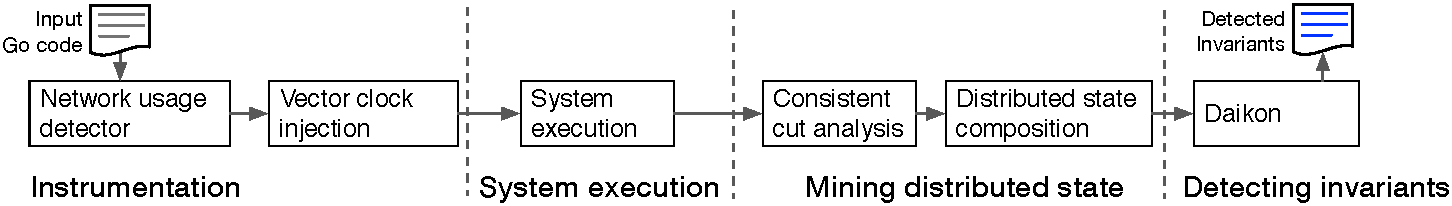
\includegraphics[width=.9\textwidth]{fig/dinv-flow.pdf}
    \caption{Overview of the steps in \dinv.}
    \label{fig:dinv-flow}
\end{figure*}

%%%%%%%%%%%%%%%%%%%%%%%%%%%%%%%%%%%%%%%%%%%%%
\subsection{System instrumentation}
\label{sec:instrumentation}
%%%%%%%%%%%%%%%%%%%%%%%%%%%%%%%%%%%%%%%%%%%%%

\dinv instruments a node's source code to produce a runtime log
containing vector-timestamped node state (each process maintains its
own vector clock).
%%   when the
%% instrumented program is executed. A log requires vector timestamps to
%% establish a partial ordering, and the values of variables defining the
%% nodes state.
Maintaining vector clocks (see Appendix~\ref{sec:formal-vector-clocks}
for the algorithm) and logging of variables require separate forms of
instrumentation.  We developed automated techniques for both.

% JS: awkward enumeration. Why not just: Protocol-handling code in
% \textit{net} remains unmodified, except for RPC share function
% signatures, which are wrapped by Dinv:...
% ... to interpose on RPC, we have built a custom codec.

\textbf{Injecting vector clocks.}
Dinv introduces vector clocks automatically by mutating the AST and by
exploiting the conventions followed by Go's networking \textit{net}
library. This library implements TCP, IP, UDP, RPC, and IPC protocols;
all of these, except for RPC, share function signature conventions which
Dinv wraps:
%% Dinv injects a custom wrapper function, and pass the original
%% function, and its arguments into the wrapper.  Within a wrapper
%% function,
vector clocks are appended or stripped from network payloads, and the
original function is executed on the instrumented arguments. For
example, a network write like \texttt{conn.Write(buffer)} becomes
\texttt{dinv.Write(conn.Write,buffer)}.  For Go's RPC, which required
a different approach, we built a custom codec. By using these two
techniques \dinv adds vector clocks to any Go program that uses the
\textit{net} library.

%%  in the background. Initializing an RPC
%% connection requires calls to the standard RPC library.
%
%% The same function capturing technique which injects vector clocks is used on
%% such calls to automatically inject the vector clock codec.
%

%%%%%%%%%%%%%%%%%%%%%%%%%
%\subsection{Logging state}
%%%%%%%%%%%%%%%%%%%%%%%%%

%%%%%%%%%%%%%%%%%%%%%%%%%%%%%%%%%%%%%%%%%%%%%
\begin{figure}[t]
    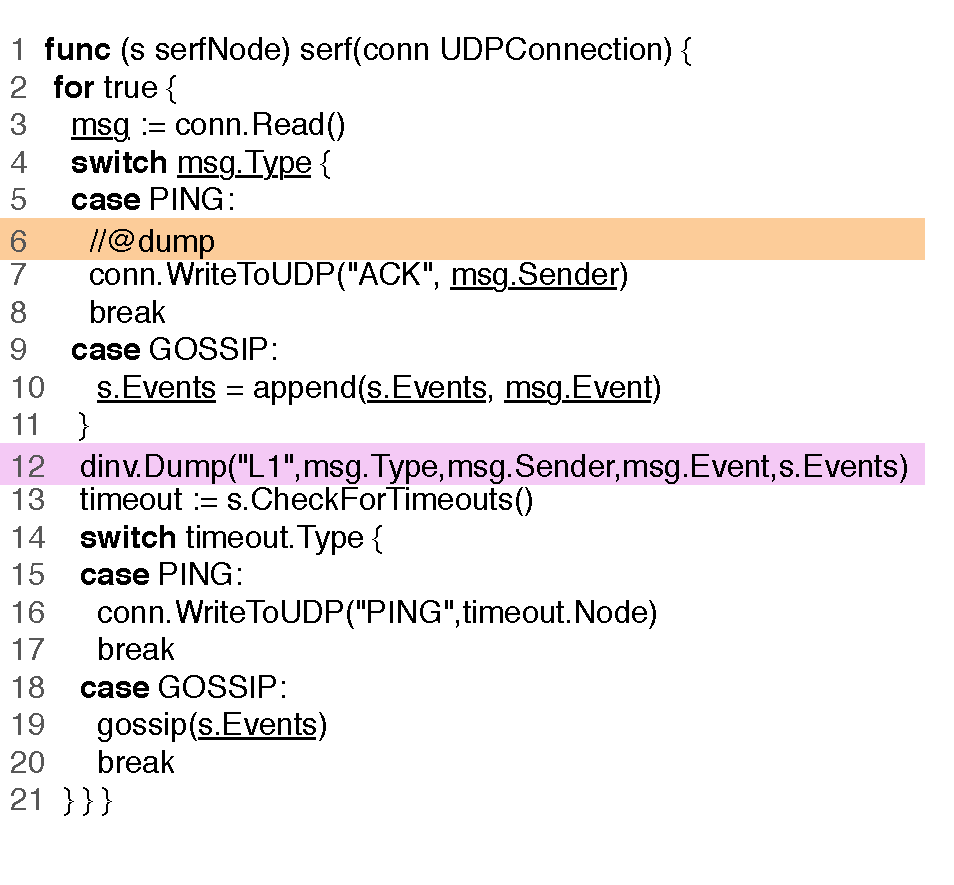
\includegraphics[width=0.50\textwidth]{fig/data-flow-3}
    \caption{Example illustrating network interacting variables
      (underlined) contained in the forward slice from $msg :=
      conn.Read()$. Two annotations on lines 6 and 12 are also
      highlighted.
      %% A dump annotation is highlighted in
      %% orange. Highlighted in magenta is logging code translated from
      %% an annotation containing networking variables.
    }
  \label{fig:data-flow}
\end{figure}
%%%%%%%%%%%%%%%%%%%%%%%%%%%%%%%%%%%%%%%%%%%%%

\textbf{Logging node state.} We designed Dinv with the assumption that
interesting state in a distributed system is composed of variables
which interact with the network. Data read from a network transitively
affects variables which interact with it, while variables which affect
the contents of network writes have a transitive influence on the
behaviour of the node that receives the message. These \emph{network
  interacting variables} influence the state of other nodes, and
properties that range over these variables capture information about
the consistency of distributed state. Dinv determines the network
interacting variables statically using interprocedural program
slicing~\cite{Ottenstein:1984, Walkinshaw03thejava}. It provides
developers with three options (Table~\ref{table:inst-strat}): (1)
automatically log these variables at all function enter/exit points,
(2) automatically log these variables at developer-annotated points,
or (3) log variables interesting to the developer at
developer-annotated points.

Dinv also allows the developer to choose between two strategies for
recording state: {\tt dump} records values at the dump statement
program point, while {\tt track} delays recording of values until
just before a network communication event. That is, track statements
aggregate state across different program scopes for a more complete
view, but they are not as precise as dump statements.

%% At each event instance a node has a distinct state and each
%% instruction that it executes potentially modifies this state.
%% %% Capturing state is an essential component of recording a log. 
%% %% , as such a complete log would contain the values of all variables
%% %% recorded after the execution of each instruction.
%% In practice, recording at this granularity is unmanageable.  Dinv
%% instead logs a subset of variables and logs these at select times.

Figure~\ref{fig:data-flow} lists partial code from Serf~\cite{serf}
that implements the SWIM protocol~\cite{das2002swim}. We will use this
example throughout the paper.
This code has two logging points in the form of {\tt //@dump}
annotation (line 6) and a \emph{paramatrized Dump} statement
(line 12). The first logs state when a \emph{Ping} is received, the
other logs state before checking for timeouts. The code also
illustrates the variables affected by a network read (underlined).
%
%% Both statements log variables within the
%% received message and the events stored on the Serf node.

%% The red highlighted variables are detected automatically through
%% static analysis by \dinv's instrumentation described in
%% Section~\ref{sec:logging-variables}, and will be logged by the
%% \emph{//@dump} annotation post instrumentation.

%% Some variables are resigned solely to local computation, and do not
%% interact with the network.  Testing invariants of such variables on
%% separate nodes would yield arbitrary results. To derive meaningful
%% distributed invariants we partition these sets of variables and
%% only log \emph{network interacting variables}, which can be
%% detected statically using program slicing~\cite{Ottenstein:1984}.
 
%%%%%%%%%%%%%%%%%%%%%%%%%%%%%%%%%%%%%%%%%%%%%
\begin{table}[t]
\centering
\small
%    \begin{tabular}{| p{2.0cm} | p{1.0cm} | p{1.0cm} |}
\begin{tabular}{ l  l  l }
\midrule
  Instrumentation strategy & \pbox{1.2cm}{Location choice} & \pbox{1.2cm}{Variables choice} \\ 
\midrule
  Entrance and exit of functions  &   Auto   & Auto \\
  User placed annotations   & Manual  & Auto \\ 
  Paramatrized logging functions & Manual & Manual \\ 
  \bottomrule
\end{tabular}
\caption{Instrumentation strategies and the control (automatic/manual)
  offered by each strategy for selecting state logging location and
  set of logged variables.}
\label{table:inst-strat}
\end{table}
%%%%%%%%%%%%%%%%%%%%%%%%%%%%%%%%%%%%%%%%%%%%%

%
% JS: Consider cutting this paragraph out for space.
%
The remainder of this section explains how the runtime node logs are
merged together, how the states of independent nodes are combined into
distributed program points, and how Dinv infers distributed data
invariants from these combined states.


%% In this section we outlined the two step procedure by which  \dinv
%% instruments a programs source code to produce a log. \dinv
%% automatically wraps network communication in order to maintain a
%% vector clock with the other nodes in the system.  Secondly, variable
%% logging statements are added using any configuration of the automated,
%% semi-automated, or manual dumping methods. In
%% Section~\ref{sec:log-analysis} we describe how the log is processed.

%%%%%%%%%%%%%%%%%%%%%%%%%%%%%%%%%%%%%%%%%%%%%
\subsection{Extracting \scc{s}}
\label{sec:log-analysis}
%%%%%%%%%%%%%%%%%%%%%%%%%%%%%%%%%%%%%%%%%%%%%

%% \item Construct a lattice structure which models all cuts of the log
%%   such that the happened-before relation is respected in each cut.

%% \item Enumerate sent and received messages for each node in the log,
%%   and reduce the lattice to cuts with no outstanding messages, the
%%   reduced lattice is the set of all consistent cuts.

%% Inferring valid distributed data invariants is a multi-faceted
%% problem. The majority of the challenges arise from concurrency. Nodes
%% which undergo concurrent state changes may simultaneously reach a
%% state which falsifies an invariant property, only to return to a state
%% in which the invariant is satisfied upon communicating again. In such
%% cases the invariant is falsified, but without a mechanism for
%% reasoning about partial ordering the property cannot be checked. The
%% following is a list of challenges inherent to checking distributed
%% invariants which our techniques address.

%% \begin{enumerate}
%% %
%%     \item The number of partially ordered \emph{events} are
%%         exponential in the number of nodes. In order to reason about
%%         the full set of partial orderings a complete model of this
%%         space must be constructed.
%% %
%%     \item Distributed state is not always resident on the nodes of the
%%         system. Analysis on distributed state is incomplete if any
%%         state is in transit.
%% %
%%     \item Distributed systems are highly variable in their both their
%%         communication patters, topologies, and node hierarchies.
%%         Determining the granularity at which to test for distributed
%%         invariants is therefore system, and property dependent.
%% %
%% \end{enumerate}
%

%% Without using any mechanism for reasoning about the order of
%% \emph{event}s in a distributed system, the number of possible
%% \emph{event} orderings is exponential. Testing invariant properties on
%% every interleaving combination of events would not only be extremely
%% costly, but also produce invariants inconsistent with the systems
%% execution. Vector clocks establish a partial ordering on events
%% between communicating nodes. However, the growth of partial orderings
%% is still exponential on events which occur between
%% communication.

%%%%%%%%%%%%%%%%%%%%%%%%%%%%%%%%%%%%%%%%
\begin{figure}[t]
    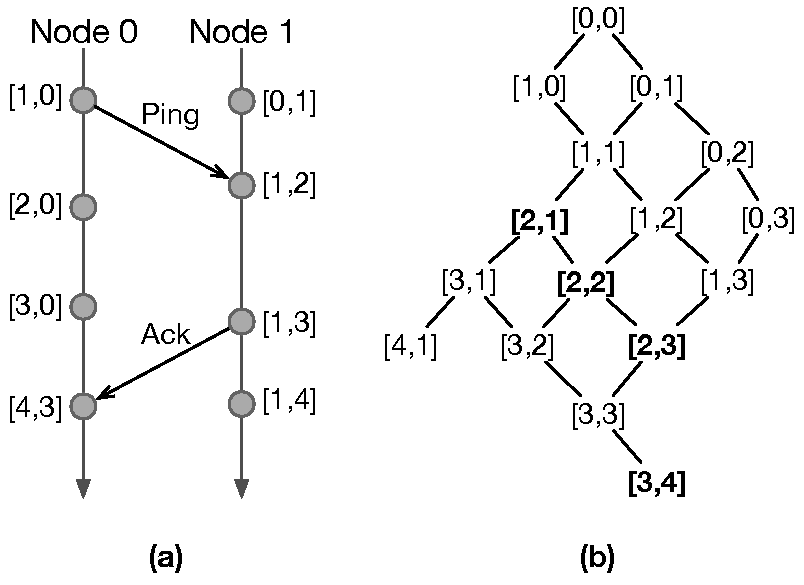
\includegraphics[width=0.50\textwidth]{fig/time-diagram}
    \caption{\textbf{(a)} Space-time diagram of an execution of code
      in Figure~\ref{fig:data-flow} with two nodes, Node 0 and Node
      1. \textbf{(b)} Lattice corresponding to this execution with
      \scc{s} indicated in bold.}
\label{fig:time-lattice} 
\end{figure}
%%%%%%%%%%%%%%%%%%%%%%%%%%%%%%%%%%%%%%%%

%% Figure~\ref{fig:time-lattice} shows a send from $H1$ at time
%% $C_{H1}[H1] = 1$ and a receive on $H2$ at time $C_{H2}[H1]=1,[H2]=2$
%% This event constrains possible event orderings.  More precisely it is
%% established that all events $C_{H1}[H1] <= 1$ happened before
%% $C_{H2}[H2] >= 2$. Therefore all ordering $C_{H2}[H2] < 2$ ,
%% $C_{H1}[H1] > 1 $ are invalid.  Such values are not part of the
%% lattice.  More formally $\forall Host_i,$ such that $Host_i$ logged a
%% clock value $C[i] = t$ all lattice clocks with value $C[i] = t$
%% Happened after the logged node event instance.

A lattice contains all event orderings consistent with the
happens-before relation~\cite{Cooper:1991:CDG:122759.122774}. This
property constrains the exponential set of potential event orderings
and supplies a complete view of a systems execution. A variety of
different algorithms for constructing a lattice have been
proposed~\cite{Garg}. Appendix~\ref{sec:lattice-appendix} presents our
algorithm for constructing the lattice.

Figure~\ref{fig:time-lattice} shows the time-space diagram and
corresponding lattice for an execution of two nodes, Node 0 and Node 1,
each of which runs the code in
Figure~\ref{fig:data-flow}. Node 0 sends a \emph{ping}, executes
two local events, then receives an \emph{ack} message.

%
% JS: scc expands to strongly consistent cut. articles missing.
%     sometimes it should be pluralized. the set of \scc{}_s_.
%
Within this lattice, \scc can be computed by enumerating sent and
received messages. We use the set of \scc in the lattice as our
granularity for inferring invariants (highlighted in bold in
Figure~\ref{fig:time-lattice}B). Merging the states of interacting
nodes at the granularity of \scc guarantees that the sum of node
states is representative of the state of the system.
Algorithm~\ref{alg:mineCuts} shows our process for extracting
consistent cuts from a lattice.

%% A variety of algorithms exist for computing consistent cuts from the
%% execution of a distributed system~\cite{MATTERN1993423}. A high level
%% description of our algorithm is given here, a full overview is given
%% in Section~\ref{sec:consistent-cuts-appendix}. We process the log by
%% enumerating sent and received messages and maintaining a delta for
%% each node. Points in the lattice on which the sum of each nodes delta
%% equals zero are to consistent cuts. This calculation is run on every
%% point in the lattice, the result is a complete set of consistent cuts.
%% Finally the states of nodes at the logical time corresponding to a
%% consistent cut are collected together. The output of this process is
%% the complete set of node states at every point during execution when
%% all state was resident in memory.

%% Figure~\ref{fig:time-lattice}B shows a lattice
%% structure of all possible partial orderings of events which respect
%% the happens-before relationship established by vector clocks.
%% We use the lattice of partial orderings as a model for accurately
%% describing a distributed execution. Algorithm~\ref{alg:lattice} is a
%% high level overview of our lattice construction algorithm.

%% Using a lattice to model distributed execution provides a complete
%% view of the execution. However, not every point on the lattice
%% is appropriate for testing invariants. Distributed state has
%% two possible locations, either resident on a node, or in
%% transit on a wire. In the latter case the state of the system
%% is unobservable.  Lattice points at which state is in
%% transmission provide only a partial view of distributed
%% state. Testing invariants at such points would be incorrect as
%% state which could falsify a property may not be
%% present. \emph{Consistent cuts} of a network are points in
%% relative time at which no messages are in transit.

%% Distributed systems are designed for a variety of purposes.  Their
%% behaviour, communication patterns, and desired invariants are also
%% highly varied. For example leader election algorithms, and
%% peer-to-peer systems typically have multiple nodes running identical
%% code, whereas client-server systems have distinct functionality.
%% Invariant properties hold at differing granularity's subject to the
%% architecture of the system. No one strategy for testing invariants
%% would detect every desired property in arbitrary systems.  Our
%% approach to this problem makes use of 3 heuristics for testing
%% invariants at differing granularity's of the systems execution.

%% In this section we describe the structures and processes we use to
%% collect the set of all consistent cuts from an execution log, merge
%% the logged states of nodes into distributed program points, and test
%% merged states for invariants. The following is a high level overview
%% of our process.

%%%%%%%%%%%%%%%%%%%%%%%%%%%%%%%%%%%
\begin{algorithm}[t]
    \KwData{A system log $L$}
    \KwResult{A set of consistent node states $S$ }
        $clocks$ := vectorClockArraysFromLogs($L$)\\
        $lattice$ := buildLattice($clocks$)\\
        $deltaComm$ := enumerateCommunication($clocks$)\\
        $cuts$ := mineConsistentCuts($lattice$, $clocks$, $deltaComm$)\\
        $S$ := statesFromCuts($cuts$, $clocks$, $logs$)\\
    \Return $S$
    \label{alg:mineStates}
    \vspace{2mm}
    \caption{High level log merging overview}
\end{algorithm}
%%%%%%%%%%%%%%%%%%%%%%%%%%%%%%%%%%%


%%%%%%%%%%%%%%%%%%%%%%%%%%%%%%%%%%%%%%%%%%%%%%%%%%%%%%%%%%%%%%%%%%%%%%%%%%%%%%%%%%%%%%%%
\subsection{Merging cuts into distributed program points}
\label{sec:merging}
%%%%%%%%%%%%%%%%%%%%%%%%%%%%%%%%%%%%%%%%%%%%%%%%%%%%%%%%%%%%%%%%%%%%%%%%%%%%%%%%%%%%%%%%

%% \textbf{Apply a merging strategy to consistent cuts to produce sets of
%%   distributed program points.}

%
% JS: ``their states and variables'', you mean the nodes'?
%     Maybe instead: To check local invariants hold on multiple nodes,
%     we merge variable states.

To check state invariants on multiple nodes, their states are merged
together and their variables are tested for invariants. All logged
states are related to the program points where they were logged.  We
therefore define a merged set of states to be a \emph{distributed
  program point}. Determining which states to merge when checking for
particular invariants is difficult because distributed systems have a
variety of communication topologies. 

For example, nodes in a client-server system execute different code,
while nodes in a distributed hash tables are identical peers whose
behaviour is dictated by their unique identifier. In each case the
system's invariant properties hold at different levels, and require
alternative views of the execution to test them. Checking that all
nodes in an election agree on a result, or that all DHT peers agree on
where to route a request requires a system wide view.  Checking that a
server responds idempotently to client requests only requires a view
between a client and the server. Checking that state updates are
propagated through a gossip protocol requires a view specific to the
dataflow in the system.

%% solutionNo one strategy for extracting distributed invariants will
%% work the desired property in an arbitrary system. Our solution is
Instead of a one-size-fits-all approach we use 3 heuristics for
merging node state for inferring invariants: (1) merge the states of
all nodes in a \scc, (2) merge only the states of unique pairs of
senders and receivers, and (3) merge the states of nodes that
participated in a totally ordered communication.
    
%%%%%%%%%%%%%%%%%%%%%%%%%%%%%%
\begin{figure}[h]
    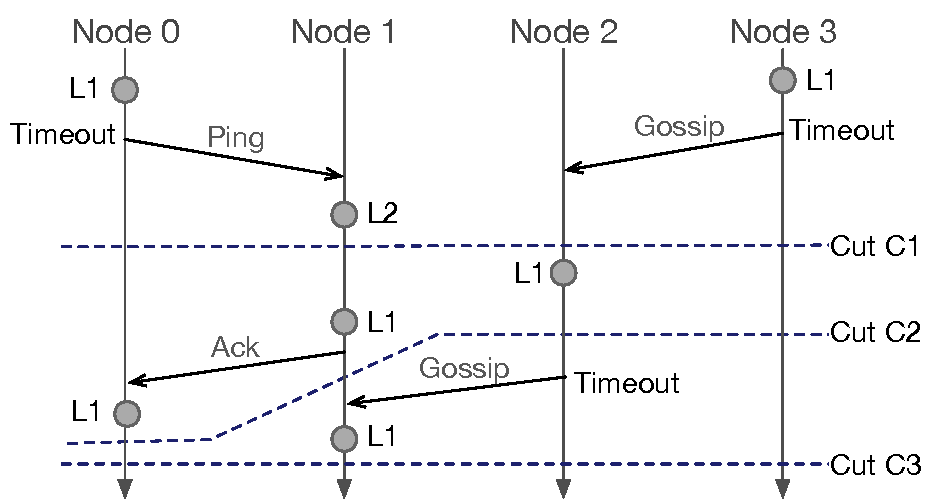
\includegraphics[width=0.5\textwidth]{fig/gossip-execution-dig}
    \caption{Sample SWIM execution with 4 nodes running code from
        Figure~\ref{fig:data-flow}. This diagram is a subset of a
        larger execution. Points $L1$ and $L2$ on each node timeline
        represent the execution of two separate logging functions. $L1$
        and $L2$ corresponds to lines 12 and 6 in
        Figure~\ref{fig:data-flow} respectivly.  Dashed lines $C1$,
        $C2$, $C3$ are \scc{s} of the execution including just these 4
nodes.} \label{fig:gossip-execution} \end{figure}
%%%%%%%%%%%%%%%%%%%%%%%%%%%%%%

%%%%%%%%%%%%%%%%%%%%%%%%%%%%%%
\begin{figure}[h]
%    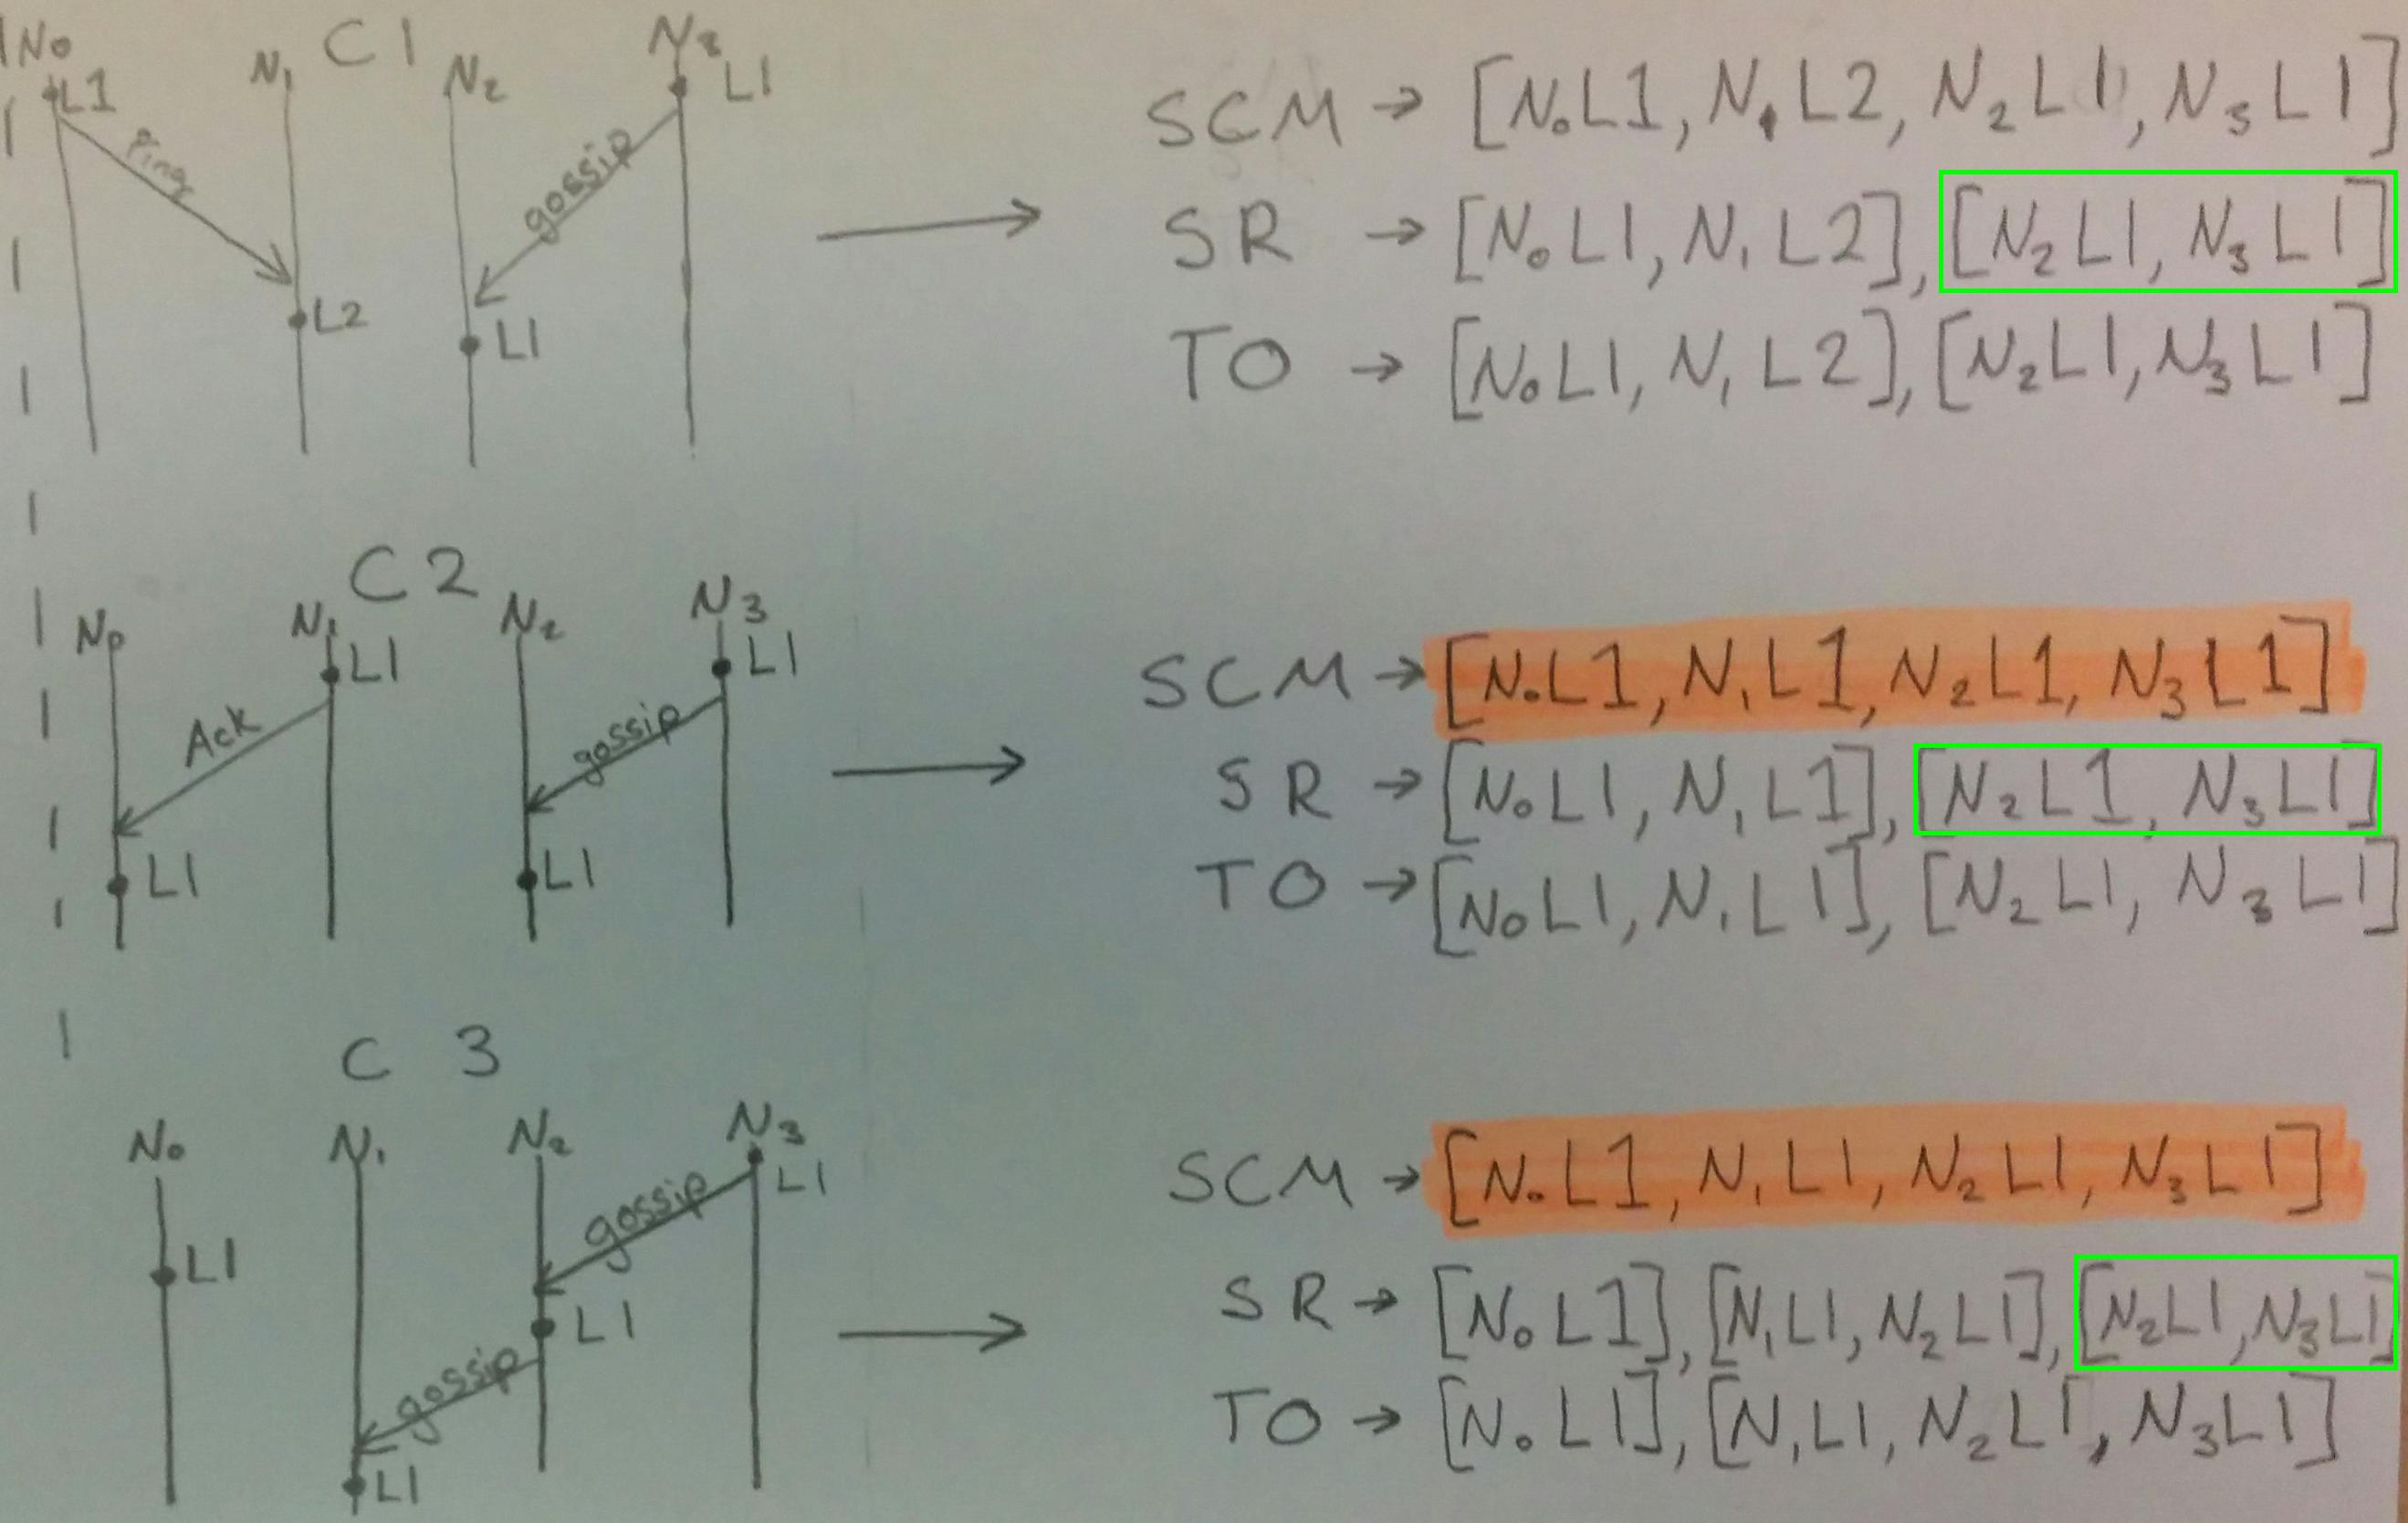
\includegraphics[width=0.5\textwidth]{fig/cuts-to-dpp}
    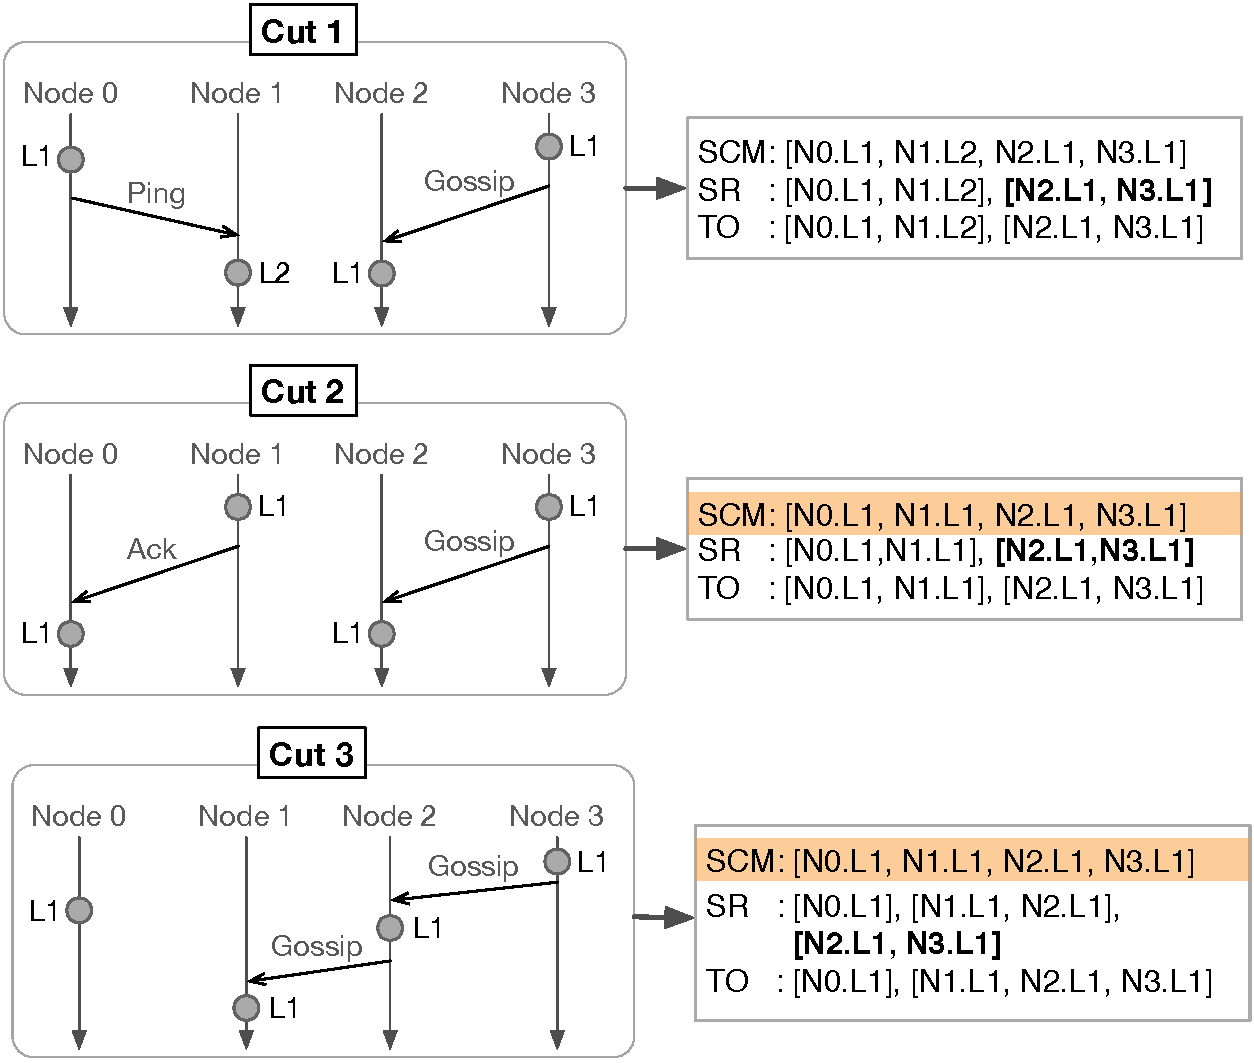
\includegraphics[width=0.5\textwidth]{fig/cuts-to-dpp-dig}
    \caption{Illustration of the three merging strategies that convert
      cuts into sets of distributed program points. On the left, are
      cuts $C1$, $C2$, $C3$ from Figure~\ref{fig:gossip-execution}
      depicted as sets of logged state. The right side shows how the
      three merging strategies, \textbf{WCM}: whole cut merge,
      \textbf{SR}: send-receive merge, and \textbf{TO}: total order
      merge, produce different distributed program points. Highlighted
      are two matching distributed programs points.}
\label{fig:cuts-to-dpp}

\end{figure}
%%%%%%%%%%%%%%%%%%%%%%%%%%%%%%

% JS: watch out for orphans and widows here.
%
\textbf{Whole cut merge.}  This merge is performed by collecting the
states of all hosts in a \scc and testing them for
invariants together.  Invariants which are true for all nodes on all
\scc are checked at this granularity. For example in a
distributed hash table where resources are not duplicated across
multiple nodes an invariant such as $\forall i,j \in nodes$ $i-keys !=
j-keys$ would be detected.  In other cases whole cut merge will not
detect invariant properties.  Figure~\ref{fig:cuts-to-dpp} shows the
whole cut merged points from a Serf execution. Checking Serf's eventual
consistency invariant with whole cut merge would not work. In the
example, if the whole cut merge distributed program point from $C1$ and
$C3$ were checked for invariants, \dinv would detect that $N_0-Events
!= N_3-Events$ because the gossip message from $N_3$ had yet to
propagate to $N_0$. Whole cut merge falsifies Serf's consistency
invariant because at the granularity of a \scc the property
does not hold.

\textbf{Send-receive merge.} In some cases it is necessary to analyze
the states of pairs of interacting nodes. In such cases merging the
states of senders and receivers in a \scc can be used to verify
invariant properties of their isolated interaction.
Figure~\ref{fig:cuts-to-dpp} details how send-receive merge constructs
distributed program points. The state of a sender immediately before a
send is merged with the state of the receiver immediately after
receiving. \textit{Cut C3} details how states are merged in cuts where
nodes both sent and received messages, as well as nodes which did not
communicate. In the case of no communication the node state is left
isolated. Whole cut merge fails to detect eventual consistency, but
the invariant can be verified with send-receive merge. In the case of
Figure~\ref{fig:cuts-to-dpp} inferring invariants over the
send-receive distributed program points would result in the invariants
$N_3-Events == N_2-Events$, $N_2-Events == N_1-Events$, and
$N_1-Events == N_0-Events$. At every instance that nodes communicate
their knowledge of events is synchronized. Therefore, the invariant
holds at a sending and receiving granularity.  Send-receive merge is
useful for detecting fine grain invariants, but because the state of
all nodes is not analyzed together the properties lack generality,
requiring users to confirm the invariant between every pair of nodes.

\textbf{Total ordering merge.} It is often useful to delineate between differing
messaging protocols between nodes. In such cases merging node states which
participate in a totally ordered interaction is useful. Vector clock values
within a \scc form a directed acyclic graph (DAG). A totally ordered
set of clock values can be extracted by starting at the most recent clock in
the cut, and backtracking along the first incident edges. When backtracking
ends at a terminal node of the DAG, the path from the most recent clock to the
terminal node, is a total ordering. The total ordering can be removed from the
cut, and what remains is a sub cut of vector clocks, which is also a directed
acyclic graph. This process can be performed iteratively to extract all total
orderings within the cut, Algorithm~\ref{alg:dpp} lists this procedure.

The set of all distributed program points is computed by running this
algorithm on the set of all \scc{s}.
Figure~\ref{fig:cuts-to-dpp} details how this merging strategy differs
from send-receive merge.  Specifically, in \textit{Cut C3} the states of
the three totally ordered nodes are merged together. Total ordering
merge has the same ability as send-receive merge to detect eventual
consistency in Serf, but it detects it in a broader scope.  In the
case of \textit{Cut C3} the invariant is $N_3-Events == N_2-Events ==
N_1-Events$.

%%%%%%%%%%%%%%%%%%%%%%%%%%%%
\begin{algorithm}
 \KwData{$State$}
 \KwResult{Set of distributed program points within a state $DPP's$}
 
 $clocks$ = $s$.getClocks()\\
 $dag$ = DagFromClocks($clocks$)\\
 \While {$dag$.Root != nil} {
     $path$ = $dag$.BacktrackFromRoot()\\
     $point$ = getHostStatesFromClocks($State$,$path$)\\
     $dag$.extract($path$)\\
     $DPPs$.append($point$)\\
 }
 \Return{$DPPs$} \\
 \vspace{2mm}
 \caption{Extract the set of distributed program points from a consistent distributed state}

 \label{alg:dpp}
\end{algorithm}
%%%%%%%%%%%%%%%%%%%%%%%%%%%%


%%%%%%%%%%%%%%%%%%%%%%%%%%%%%%%%%%%%%%%%%%%%%%%%%%%%%%%%%%%%%%%%%%%%%%%%%%%%%%%%%%%%%%%%
\subsection{Bucketing distributed program points by type}
%%%%%%%%%%%%%%%%%%%%%%%%%%%%%%%%%%%%%%%%%%%%%%%%%%%%%%%%%%%%%%%%%%%%%%%%%%%%%%%%%%%%%%%%

%% \textbf{Bucket distributed program points based on nodes they include
%%   and the variables they contain.}

To derive arbitrary invariants multiple instances of variables and
their values are required. Properties which hold on all instances are
invariant. To test invariants on the state of two or more nodes the
combined set of variables must be identical in each instance that an
invariant is tested. Testing invariants on instances with
non-identical sets of variables would identify correct invariants on
the intersection of the sets, and potentially incorrect invariants on
the sets symmetric difference.  Because of this we only test
invariants on identical sets of states.

The final process to prepare the logs for Daikon is to bucket
distributed program points together.  Distributed program points are
identifiable by the triple \emph{(nodeid, source, loc)} of the logging
statements from which generated them, and the set of nodes from which
are merged.  Figure~\ref{fig:cuts-to-dpp} highlights two distributed
program points generated by whole cut merge from different points in
Serf's execution, which would be bucketed together.  The points
emphasized in bold generated by send receive merge correspond to the
same distributed program point merged from separate cuts, these points
are also bucketed together.  We consider all \textit{Dump} statements to be
unique as they do not necessarily contain the same set of
variables. Therefore, regardless of merging strategy, the number of
different buckets generated can be exponential in the number of
\textit{Dump} statements. \textit{Dump} statements provide a precise
view of particular functionality, but also cause an output explosion.
%
% JS: each statement into one? one what. The result of what?
%
\textit{Track} consolidates each statement into one, the result is a
collapse of exponential output at the cost of precision.  For example
using whole cut merge and 2 \textit{Dump} statements on a log of 4
nodes results in a total of 16 distinct distributed program points,
whereas \textit{Track} in conjunction with single cut merge results in
1 distributed program point. This exponential reduction is true for
all merging strategies.
%
% JS: watch out for widow
%

% JS: Using their id's as identifiers. redundant. Are you saying you're
%     using identifiers as a key in the bucket?
The bucketing algorithm is as follows: distributed program points are
placed into buckets using their id's as identifiers.  Finally each
bucket is written to a separate file for analysis by Daikon.

%\todo{add an example of bucketing}


%%%%%%%%%%%%%%%%%%%%%%%%%%%%%%%%%%%%%%%%%%%%
\subsection{Using Daikon to infer invariants}
%%%%%%%%%%%%%%%%%%%%%%%%%%%%%%%%%%%%%%%%%%%%

Daikon is a tool to dynamically detect likely data
invariants~\cite{Ernst07}.
%
We use a Daikon on the logged concrete values in each bucket to infer
invariants.
%
Daikon infers likely data invariants based on data traces, referred to
as \emph{dtraces}.  The result of running \dinv on a log, is a set of
\emph{dtraces} for each unique distributed program point present
during the systems execution.  \dinv output a dtrace file for each set
of matching distributed program points.  Daikon is run on each
\emph{dtrace} to detect invariants at the corresponding point,
Daikon's output is a set of invariants with variables prefixed by the
nodes id, source file, and line of code on which they were present to
distinguish them from one another. 

\iv{Have to describe mechanisms inside of Daikon for handling spurious
  invariants.}

\iv{Have to note somewhere (here?) that more executions that are
  diverse improve the quality of the mined invariants.}

Appendix~\ref{daikon-appendix} details Daikon's approach to
invariant detection, and our methodology for translating Daikon
invariants into first order logic.



\section{Proof of Concept System}
\label{sec:implementation}
To evaluate the practicality of the aforementioned design we built a simple proof-of-concept tool operating entirely on IPv6 memory addressing. The implementation is minimal and focuses on appropriate conversion and network transport techniques to demonstrate the basic IPv6 shared memory use case and its benefits. The virtual memory system as well as the control plane and consistency management properties of the BlueBridge design are left as future work.
The client-server program is written in C and Python and utilizes basic C memory operations.
\subsection{System Aspects}
% The general operational structure of the tool is already reminiscent of the full design proposal.
The client consists of a library of simple remote allocate, read, write, and free functions which are mirrored on the server side. Allocation is chosen at random out of a list of possible host numbers. Instead of \texttt{mmap()}, the client stores acquired pointers in a simple list structure to read and write its data. When accessing remote memory the client inserts the IPv6 pointer into the header and sends it using a Linux datagram socket. The server retrieves the destination IP section, converts the 128 IPv6 address into a 64 bit pointer, and faithfully performs the requested action. We currently do not check for invalid or corrupted pointer addresses, which may lead to errors on the server side. A fully asynchronous, non-blocking client and server programs as well as checking pointer addresses are functions left for future work

\subsection{Networking Aspects}
We run our proof of concept system in Mininet~\cite{mininet}, a networking virtualization engine primarily used for SDN research.
% It enables the testing of networking configurations on a single machine by encapsulating nodes in a custom, dedicated network container.
% Mininet supports virtual switches as well as custom controllers, making it a prime candidate to conduct our tests.
Our current network setup consists of a single switch and controller managing up to 42 nodes. We are running a simple Open vSwitch which is pre-configured over several static \texttt{add-flow} commands which specify the appropriate server subnets. 
% Although the system is capable of running in conjunction with a controller (here: Ryu), we are not yet relying on it. The controller would only operate in reactive mode and not install any routing entries. 
All forwarding is performed on layer two only and all flow entries are MAC-based. As these type of operations can be just as effectively covered by the static configuration, we have decided to not include the controller in this prototype.We leave controller integration to future work.

We still rely on the Linux network stack for communication, which automatically configures all necessary operations below transport layer. This includes neighbor discovery, packet construction, route entry management, and packet forwarding.
Every pointer is a unique IPv6 address and hosts do not reply to unknown addresses. As a consequence, our system needs dedicated routing table entries for each node and utilize the network discovery protocol to function properly.
As it is impossible to specify IPv6 subnet proxies natively, every node runs a NDP-proxy server which responds to NDP solicitation requests. For every pointer that is sent out into the network, a NDP solicitation request is broadcast. The proxy of the owning server will respond and the appropriate routing entry is created on all relevant nodes.
This behaviour is highly undesirable as it generates round-trip overhead, nearly doubles network traffic, and may lead to peculiar problems (see Section~\ref{sec:silly_ndp}). It is thus mandatory to abolish the dependence on NDP for our system to succeed. As it is a default feature of Linux transport layer operations, we are planning to move to raw socket programming entirely. This also provides us with the benefit of high customizability and the potential to define a leaner, specialized protocol.

\subsection{IPv6 Remote Paging}
% \ac{Amanda please work on.}
% \ac{Done to be similar to DSM systems work, see \cite{Protic1996}}
We also created a \texttt{userfaultfd} program to perform remote paging, reminiscent of how DSM systems would transparently retrieve remote memory for an application. When a page fault occurs, the system determines if the page is remote or local. If the page is remote, it performs whatever communication is necessary to retrieve it, if it is local, it fetches the page. \cite{Protic1996} In our implementation, we moved most of the \texttt{client} logic into \texttt{userfaultfd}. The program \texttt{mmap}s $n$ number of addresses into memory marked to be handled by the \texttt{userfaultfd} handler. When it \texttt{mmap}s the memory, it allocates remote memory on the \texttt{server} and maintains a mapping of local addresses to remote addresses. Every access causes a page fault which is handled by our handler. We then forced page fault accesses to these pointers. For each page fault, the program checks to see if the pointer is remote or not by checking a hardcoded map. If the pointer is remote, it performs a READ operation on the remote memory and loads that into the local pointer.

% After building the program we conducted several tests to evaluate its current efficiency and to identify potential shortcomings and bottlenecks.

\section{evaluation}
\label{sec:eval}
We measured various performance aspects of Camelot to measure its
scalability and competitiveness with existing data processing
platforms. We developed a set of benchmark programs with diverse
memory access patterns, to measure the quality of our page eviction
strategies, threading performance, and raid overhead.

\subsection{Experimental setup}
Our tests were performed in the Mininet~\cite{mininet} as well as on real hardware.
Mininet is a host-local network emulator intended to rapidly prototype SDN and data center network environments. Mininet allow us to verify and deploy code quickly, without having to worry about hardware constraints or configuration. While absolute performance may not exactly be accurate, relative improvements are generally reliable. 
Our real hardware setup consisted of three servers, each of which is equipped with a 10-Gigabit X540-AT2 NIC, 32 GB of memory, and two four-core Intel(R) Xeon(R) E5-2407 v2 CPUs. The cores do not support hyperthreading.
The microbenchmarks and threading tests were performed on real hardware to provide an accurate picture of the current system efficiency. The remaining tests were run in Mininet, as absolute performance was not of concern.

\subsection{Threading Performance}
To understand the implications of multithreading, and to verify the functionality of our current networking stack, we conducted several microbenchmarks. We pinned each thread to one core in a round-robin fashion, as this approach has proven itself to be more stable and reliable during testing. Our benchmark consisted of a million read and write requests, which we then scaled up to 64 threads. The results are shown in Fig~\ref{fig:threads}.
As expected, throughput scales linearly up to eight threads and latency does not increase. Unfortunately, the program is unable to exhaust the NIC bandwidth and only reaches around 3.5 out of 10 Gbit per second. At the same time, while latency in Mininet is on the order of ~9-10 microseconds, real RTT is ~60-70. This caused by a lack of request batching and the use of slow kernel networking code.

We decided to go beyond the expected scaling of eight cores and explore the system behaviour up to 64 threads. The pinned experiment ran stable, demonstrating a reasonable reliability. The throughput results exhibit a sawtooth pattern, with a local maximum occurring  every eighth thread. This pattern is caused by the number of cores and pinning. However, this does not explain the maxima achieved by 16 and 24 threads. We assume that these may be caused by batching of requests in the NIC buffer, which is beneficial for throughput.
Latency behaves as expected, with a mild increase in early iterations that transitions into wild instability the more threads are added.

\begin{figure*}[H]
    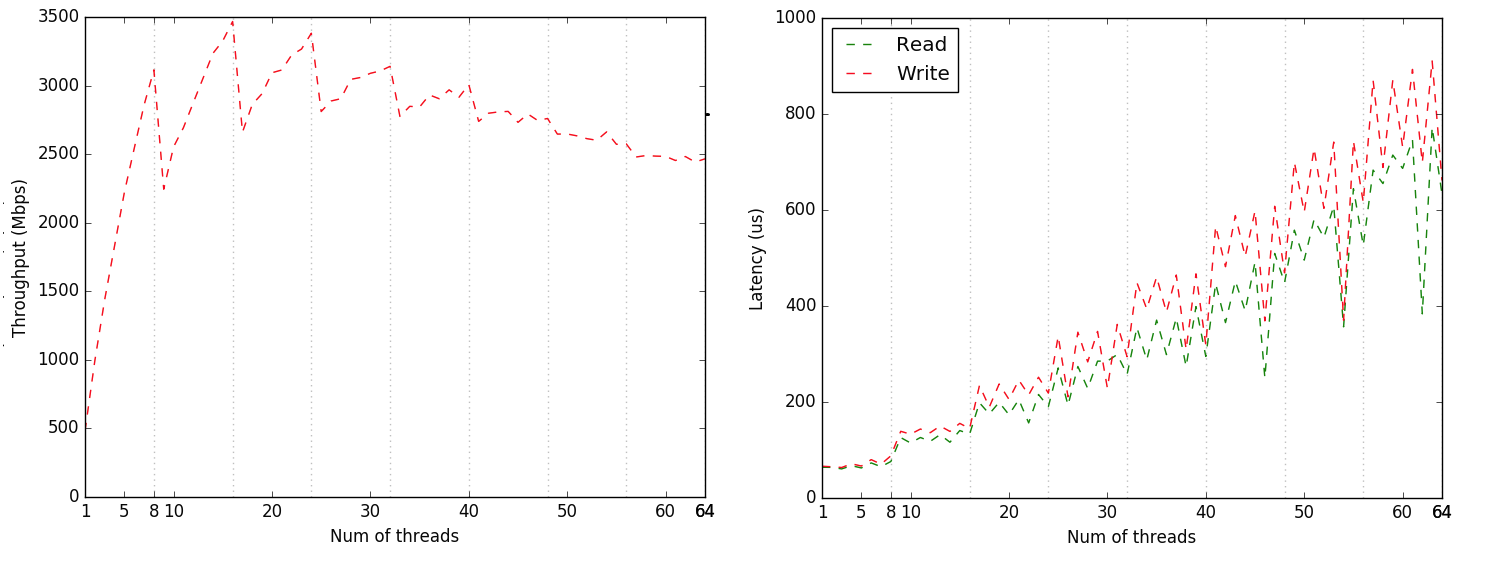
\includegraphics[width=\textwidth]{fig/threads_pinned}
    \caption{Microbenchmarks of the Camelot request API. The two figures show latency and throughput with threads pinned to cores in round-robin fashion.}
    \label{fig:threads}
\end{figure*}

\subsection{Paging Performance}
The purpose of our page performance evaluation was to quantify the performance improvement over the BlueBridge paging policy and to determine which paging policy is most efficient. Our first benchmark was running PageRank with varying amounts of local memory and each paging policy. The entire runtime is measured on the Google web graph dataset, roughly 75MB. The second benchmark was sorting a large number of random integers with varying local memory amounts.

\begin{figure}[H]
    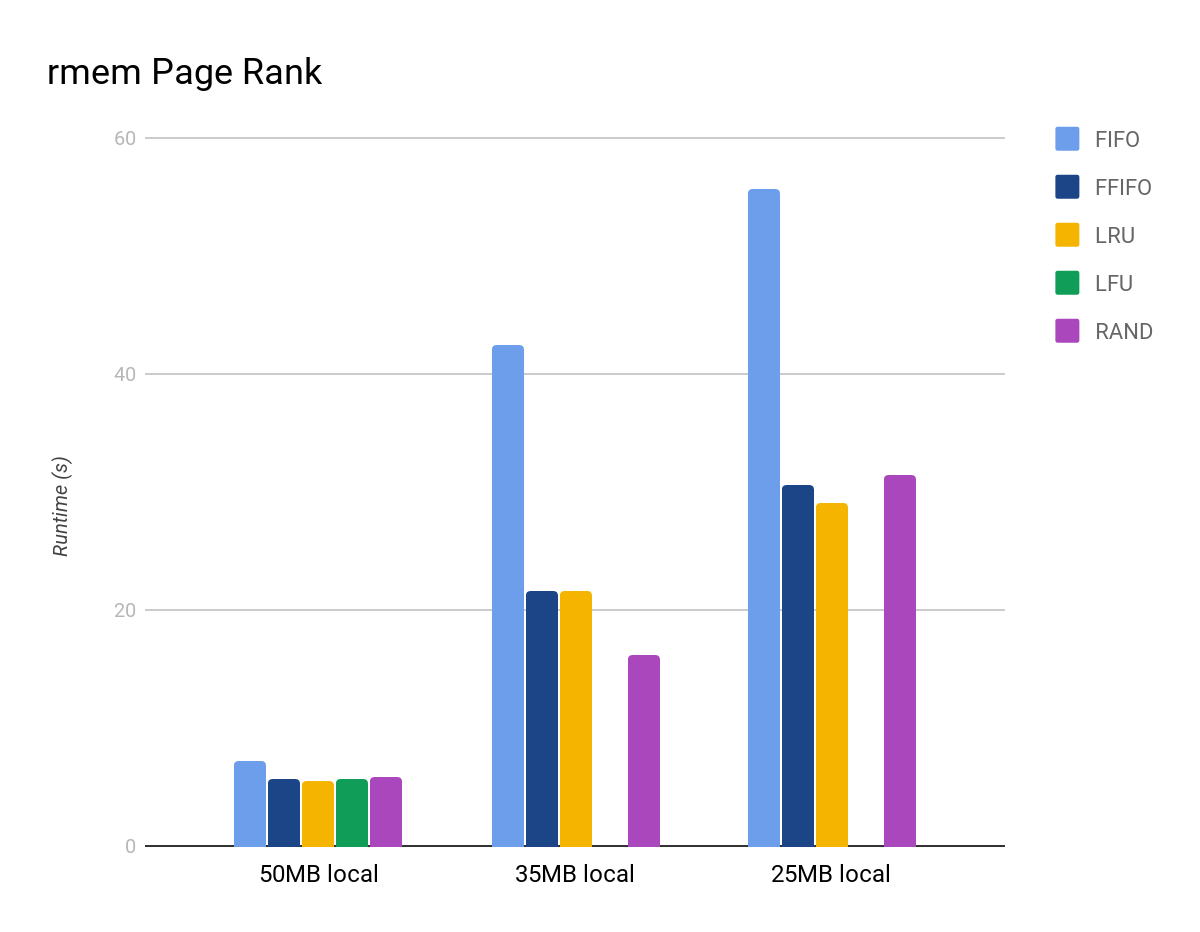
\includegraphics[width=\columnwidth]{fig/policyPerformance}
    \caption{PageRank runtime benchmark for each policy with decreasing amount of local memory.}
    \label{fig:policyPerformance}
\end{figure}

In the Pagerank benchmark, the LRU and improved FIFO policies outperformed the existing FIFO regardless of local memory size, achieving nearly half the execution time in the 35MB and 25MB tests as shown in Fig~\ref{fig:policyPerformance}. As local memory was limited and more page replacements were made, the LFU eviction policy failed to replace the correct pages and execution time increased dramatically, the results of which for 35MB and 25MB local memory were 9 minutes and 40 minutes respectively. To test the effectiveness of the policies, a random replacement policy was implemented. Ideally there would have been a substantial performance benefit from using the new replacement policies over the random replacement but the random replacement policy performed the best in the 35MB local memory test and still performed reasonably well with 50MB and 25MB. This is could be due to the policies implemented being based only on write usage as the nodes are moved around on segfault. For further work it would be beneficial to capture the read usage in an efficient way for the LRU and LFU policies.

\begin{figure}[H]
    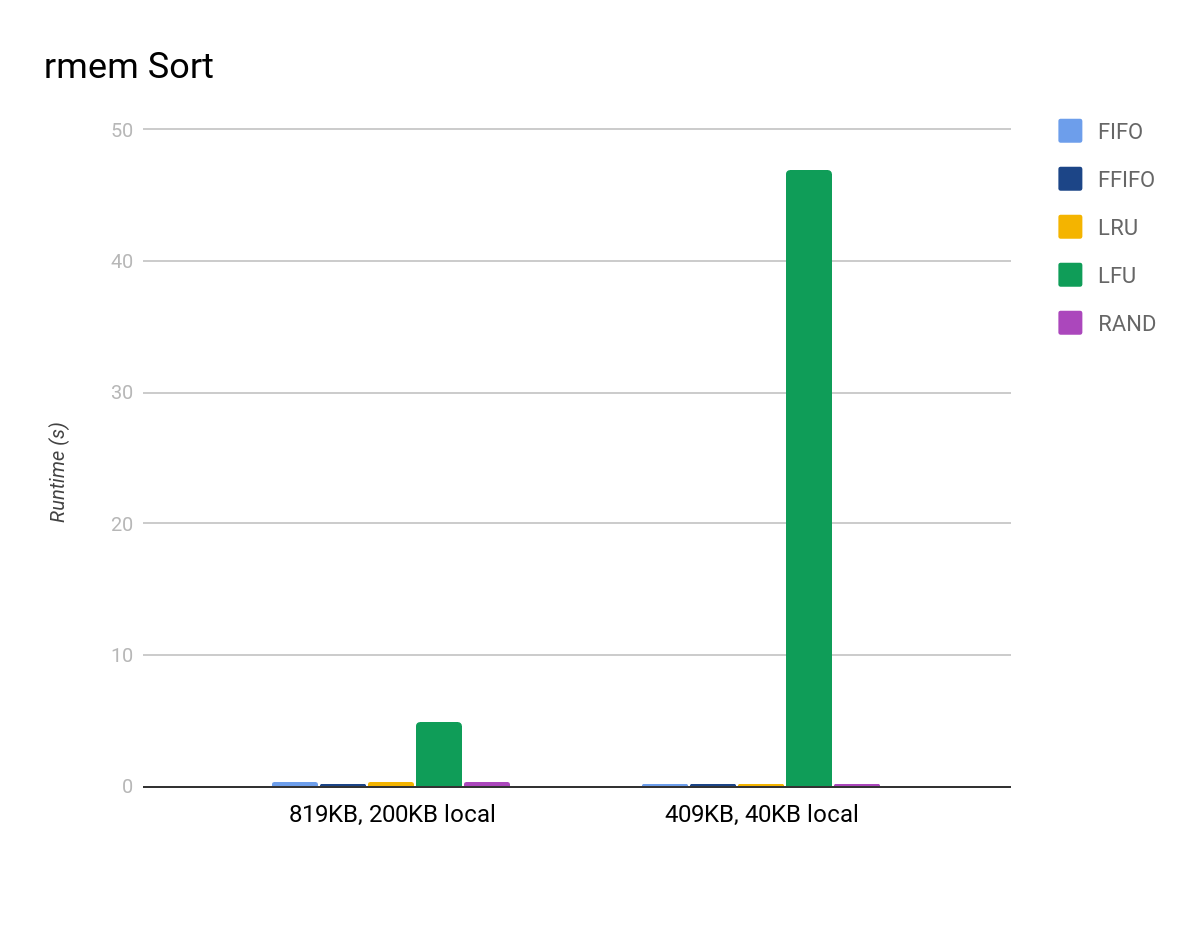
\includegraphics[width=\columnwidth]{fig/sortPerformance}
    \caption{Sort runtime benchmark with decreasing amount of local memory for each policy.}
    \label{fig:sortPerformance}
\end{figure}

In the Sort benchmark the existing FIFO and new replacement policies performed similarly with the exception of LFU. The results of the Sort benchmark in Fig~\ref{fig:sortPerformance} show the extreme difference between having a large number of local pages and a small number of local pages when using LFU.

\subsection{RAID Overhead}

Our goal in evaluating our RAID implementations is twofold. We first
wished to establish a baseline overhead of running raid over regular
remote memory, and to compare the cost of parity calculation relative
to the no parity case common to RAMCloud. In both cases we found that
the size of local cache used dramatically affected performance, so we
report our performance results as a function of local cache size. We
measured relative performance of these algorithms by timing
iterations of a single threaded PageRank algorithm. Each iteration
of page rank requires both a read and write step, so in each
iteration all pages are read, and written to remote memory.

\begin{figure}[H]
    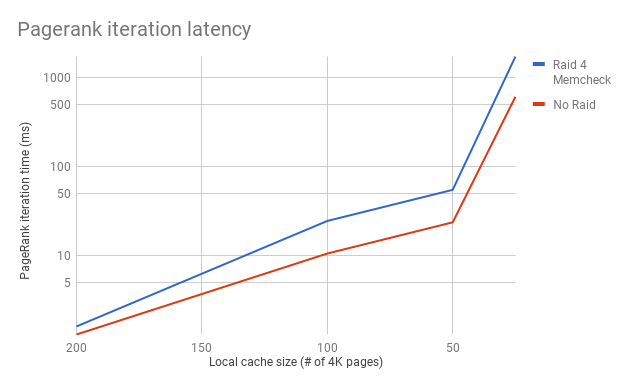
\includegraphics[width=\columnwidth]{fig/Raid4Overhead}
    \caption{A logarithmic plot of RAID 4 running with memory check performed on reads, and parity calculations on writes, v.s traditional remote memory.}
    \label{fig:raid4Overhead}
\end{figure}

We found that running RAID4 with memory correction on a small local
cache 1-2\% of the entire graph) caused a 2x slowdown in PageRank
iterations. The relation between performance and local cache size is
plotted in Figure~\ref{fig:raid4Overhead}. As the number of local
pages was increased to 10-20\% of the entire graph the overhead was
reduced to ~1.5x slowdown. A large component of this overhead, is not
the cost of performing XOR, it is due to our networking stacks lack of
optimization for RAID. Our RAID manager is build directly on top of
our remote memory stack, which issues single requests in the form of 4K
pages. Therefore RAID 0,4,5 increase network bandwidth by $(n-1)x4K$
per page. Batching requests, and optimizing the network stack to
read/write stripes of pages will substantially drop overhead.

\begin{figure}[H]
    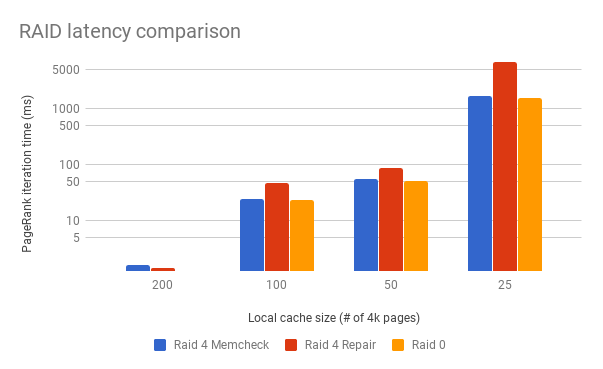
\includegraphics[width=\columnwidth]{fig/RaidComparison}
    \caption{Raid 4, Raid 4 with failure, and Raid 0 vs local cache size}
    \label{fig:RaidComparison}
\end{figure}

To evaluate the relative performance of RAID 4 \& 5 compared to RAID
0 \& 1 we likewise measured PageRank iteration times. We found that
Raid 4 and 5 introduce a 6\% overhead on both RAID 0 \& 1, and that
the overhead was directly proportional to parity calculation time.
Figure~\ref{fig:RaidComparison} plots our comparative results. RAID 0
\& 1 ran competitively within 0.01\% of each other. The only notable
difference between then was the lack of a need for RAID 1 to wait for
stragglers on reads. Given our setup the straggler problem was
unobservable to our measurements. RAID 4 \& 5 operate identically from
a latency and bandwidth perspective. We also measured the performance
penalty from running during a failure. We killed a single memory
server while running PageRank and observer the overhead to be
approximately 2x. The majority of the overhead was caused by waiting for
a preset 100 microsecond timeout to fire and initiate the repair
calculation. This overhead could be reduced by introducing a failure
detector which would initiate repair immediately. In this case the
overhead of running Camelot on 3 memory nodes under failure, vs
RAMCloud is 6\% while requiring 50\% of the total memory.


%%%%%%%%%%%%%%%%%%%%%%%%%%%%%%%%%%%%%%%%%%%%%
\section{Discussion}
\label{sec:discussion}
%%%%%%%%%%%%%%%%%%%%%%%%%%%%%%%%%%%%%%%%%%%%%

\textbf{Using Dinv.} Dinv infers invariants that are \emph{likely}
because it is a dynamic analysis approach that only considers some
finite set of system behaviors. The inferred invariants are not a
verification of the system.
%
But, Dinv is pragmatic when considering today's software development
practices that include widely used dynamic analyses like testing.
%
Unlike testing Dinv helps developers understand what happened. Dinv
can be extended towards testing by having developers assert expected
Dinv-inferred invariants for a set of curated executions.

%% standard practice. Moreover, Dinv can actually augment the results of
%% test runs.

%% we were able to observe it under real
%% world conditions (long runs, failure scenarios) without needing a
%% complete specification of it's behavior.
%% %
%% Dinv allowed us to refine and narrow the instrumentation iteratively
%% based on actual execution results.

To use Dinv a developer must have access to the system's source code,
and they must be familiar with the system. In our evaluation we considered
four large distributed systems, none of which we were familiar with
prior to this study. In each case we used all of the resources
available to us (papers, source code, documentation) to understand the
desired system properties and to interpret Dinv's output. We have not
carried out a formal usability study on Dinv, but we do have some
anecdotal evidence that it is not difficult to use: students with no
prior distributed systems background successfully used it in a
graduate distributed systems course. 

%% Its' behavior, which is often not
%% thoroughly documented, must be translated into \emph{likely
%%   specifications} that we can infer.
%

Depending on design of the system distributed state may be difficult
to identify and encode, particularly when this requires reasoning
about program paths that lead to network actions.
%
As we had no prior knowledge about the four systems in our evaluation
and were successful in inferring interesting properties we are
confident that with proper training developers would be able to
similarly instrument their systems.
%
% However, the catch is that the developer must be willing to and is
% sufficiently familiar with their system to interpret \emph{likely
%  specifications} that we infer for their system.

\textbf{Merging strategies.} Dinv's three merging strategies
(Section~\ref{sec:merging}) were motivated by our evaluation
experience. These cover different views on the systems and allow Dinv
to detect a wide range of invariants, from properties true across all
hosts during the entire execution, to eventual consistency properties
observed on the level of send-receive pairs. Even so, these strategies
are not exhaustive. All three merging strategies were implemented in
less than 15 LOC; we therefore think that custom merging strategies
offer a reasonable way to extend Dinv.

%% The lattice structure provides all data necessary for different
%% analysis approaches.

\textbf{Daikon templates for distributed system invariants.}  Daikon
is designed to infer invariants for program points in a sequential
system. Dinv uses Daikon by presenting it with a synthetic program
point that actually corresponds to a distributed state. This approach
has its limits. In particular, Daikon supports a fixed set of
invariant templates that at most describe 3-ary relations. %This is
%insufficient for mining invariants like the one given earlier:
For an invariant mentioned earlier, $coordinator.commit =
replica_i.commit$ for each replica $i$, Dinv mines as many individual
invariants as there are replicas in the system.
%
%Another approach 
%is to extend Daikon invariant templates to be 
%
We experimented with adding support for n-ary properties to Daikon and
see promising results. These properties would help to compactly
describe properties of larger systems, like those with many nodes.
%% We also added an invariant while
%% trying another approach to checking eventual consistency, by showing
%% that at each point the difference in state between hosts is bounded.

\textbf{Analyzing executions containing failures}. A major challenge
for distributed systems is dealing with failures. In our experiments
with the SWIM protocol in Serf we have shown that Dinv can establish
properties of a system during network partitions. However, in general,
Dinv is limited in the kinds of system failures it can be used to
study.
%
\dinv's decision to split the execution into strongly consistent cuts
and translating the happens-before graph into a lattice structure
assumes a relatively stable execution environment. For example, a run
with a network partition that is not resolved before the end of
execution, may not result in any cuts from the point where the
partitioned occurred. Supporting other failure cases may require
changing \dinv's analyses; a nuanced, but feasible project.

%% , we were able to extract useful knowledge from
%% executions with network failures.
%

%% On the other hand, infrequently communicating nodes will force the
%% lattice to fan out during log analysis which often set's an upper
%% bound on the number of analysed hosts for performance reasons. Further
%% code optimization of \dinv or the application of more advanced
%% algorithms might alleviate this problem. We didn't feel our analysis
%% to be limited by the number of nodes behind a reasonable threshold.

%%%%%%%%%%%%%%%%%%%%%%%%%%%%%%%%%%%%%%%%%%%%%
\section{Related work}
\label{sec:related}
%%%%%%%%%%%%%%%%%%%%%%%%%%%%%%%%%%%%%%%%%%%%%

%% Popular tools for collecting and analyzing console logs include
%% fluentd~\cite{fluentd}, logstash~\cite{logstash},
%% graylog~\cite{graylog}, splunk~\cite{splunk},
%% papertrail~\cite{papertrailapp}, loggly~\cite{loggly}, and
%% sumologic~\cite{sumologic}.

Distributed system state has a long
history~\cite{dist_snapshots_Chandy1985,
  state_machine_replication_Schneider1990,
  geels_friday_nsdi_2007}. Prior work uses concrete state of a system
to check the system against known properties~\cite{yang_modist_nsdi09,
  killian_macemc_nsdi_2007}. To be more immediately useful to
developers who are attempting to understand complex systems, we think
that distributed state requires abstraction. Dinv is one way to
achieve this abstraction.

\textbf{Mining distributed systems information.}
%
At its core DInv is a tool to mine information about a distributed system.
%% tackles the problem of mining and abstracting distributed state.
Other work in this domain detects
dependencies~\cite{lou_mining_distsys_deps_osr_2010}, temporal
properties~\cite{Beschastnikh2012},
anomalies~\cite{xu_console_log_mining_sosp_2009}, and performance
bugs~\cite{Sambasivan11}. However, this prior work focuses on events,
and not state. The closest prior work in the sequential domain is
Daikon~\cite{Ernst07}, which cannot be applied to distributed systems.

Yabandeh et al.~\cite{yabandeh_avenger_srds_2011} infer
almost-invariants in distributed systems: invariants that are true in
most cases and assume these invariants only are violated due to
bugs. They require the user to provide a list of variables and
functions for invariant inference. DInv can infer distributed state
variables automatically. They also assume that an external module
generates a trace of globally consistent cuts with distributed state
for their algorithm; our approach actually instruments the system and
generates these consistent cuts.

%% Temporal invariants in distributed systems have been automatically
%% inferred by mining partially ordered logs
%% Finite state machines, and communication finite state machines can be
%% automatically detected using similar
%% processes~\cite{Beschastnikh13}~\cite{Beschastnikh14}. Both approaches
%% require minimal instrumentation and summarize useful state information
%% for developers.  These high level approaches do not attempt to detect
%% data properties.

%% Distributed system analysis is a rich field with many contributions
%% aimed at profiling distributed system behaviour.


\textbf{Other analysis of distributed systems.} Dynamic analysis of
distributed systems has yielded a number of tools to aid
developers. Googles Dapper~\cite{Dapper} analyzes traces of
distributed systems to produce call graphs and report performance
information. 
%% The system is widely used at Google and has been credited
%% with large scale improvements to AdWords. Dapper does not focus on
%% distribute state.
%
%% Dapper is not fully automated and requires developers to
%% manually annotate source code to produce trace files.
%
Another profiling tool, \textit{lprof}, developed by Zhao et
al.~\cite{Zhao:2014:LNR:2685048.2685099} automatically instruments
Java bytecode by injecting information method information into
existing log statements. Based on the generated execution logs lprof
builds a call graph and infers temporal properties about the
log. Lprof's instrumentation relies on synchronized timestamps rather
then vector clocks, which limits its applicability to distributed
systems.
%% generality of the system. Both approaches have proven useful as
%% debugging aids, and for identifying latency issues.

%% There have been prior efforts to automatically instrument networked
%% systems, and derive their invariants using
%% Daikon. InvarScope~\cite{groeneveld2010automatic} detects invariants
%% in JavaScript applications. 
%% %% Their technique involves capturing HTTP request and instrumenting
%% %% them on the fly. They then profile an entire site by merging the
%% %% invariants found on a large set of runs.
%% This approach is localized to client-side code, and does not
%% generalize beyond client-server systems.
% detect global invariants between the client and server.

%% Real time monitoring of distributed systems is classically hard due to
%% variances in network topologies, and correlation between events on
%% various machines.
%% Dtrace~\cite{Cantrill04dynamicinstrumentation}, and
Monitoring systems such as Fay~\cite{Fay2011} and Pivot
tracing~\cite{Mace2015} use dynamic instrumentation for real-time
diagnosis of distributed systems by activating trace points at
runtime. %% Unfortunately correlating events
%% using these programs is still a complex developer task. Pivot
%% tracing
%~\cite{Mace2015} addresses this problem by introducing a
%% happens-before join which enables trace queries to be contextualized
%% by Lamport's happened-before relation. All these approaches have the
%% advantage of introducing minimal overhead to running systems while
%% providing diagnostic information. 
%% The processing of information generated by the traces is a task left
%% to developers. 
These tools do not infer properties, such as invariants, that are
present in the traces they capture.

\textbf{Formal methods for distributed systems.}  %% Although recent
%% experiences from Amazon~\cite{newcombe_tla_cacm15} indicate that there
%% is utility in modeling existing implementations,
%% We assume that developers want to check their implementations, not a
%% formal model, which is also difficult to create.
%
Unlike recent methods that use theorem proving to synthesize correct
systems by construction~\cite{wilcox_verdi_pldi15,
  hawblitzel_ironfleet_sosp2015}, our work is immediately applicable
to existing production systems. %, specifically those written in Go.
%
Previous work also considers checking existing system implementations
directly~\cite{yang_modist_nsdi09, killian_macemc_nsdi_2007}, or
checking system properties at runtime or during program
replay~\cite{reynolds_pip_2006,
  geels_friday_nsdi_2007,liu_d3s_nsdi_2008,VeriFlow}.  This work
assumes that a developer can, and is willing to, specify properties of
their system. By contrast, Dinv does not require the developer to
formally specify their system and aims at elucidating the runtime
properties of the system.

%% However, the catch is that the developer must be willing to and is
%% sufficiently familiar with their system to interpret \emph{likely
%%   specifications} that we infer for their system.

%% Notable progress has been made in summarizing specifications via
%% symbolic message sequence graphs to group machines into classes based
%% on similarities in their communication patterns~\cite{Kumar2012}. This
%% process is out of the scope of our work but could be leveraged to
%% yield more specific invariant inference.

%% \todo{Other papers to cite:
%% Avenger SRDS,
%% \url{http://arxiv.org/pdf/1604.04638.pdf}
%% \url{http://ieeexplore.ieee.org/xpl/articleDetails.jsp?arnumber=7381842}
%% }

\section{Conclusion}
\label{sec:conclusion}

We have shown and discussed a new version of DSM which leverages in network
management to expose a NUMA machine to the user. This provides a simple
generic interface for the developer to program on, yet still provides the
benefits of distribution of data and compute. We describe the Camelot system,
which builds upon the BlueBridge system by adding multi-threading support,
different paging policies, and RAID for memory fault tolerance. We evaluated
each additions' performance impact and functionality. In our current setup, Camelot was able to scale 
up to eight cores, achieving a throughput of 3.5 Gbps with an average request latency of around 60 
microseconds. In memory RAID cost a 6\%overhead in computation, but required half of the memory of RAMCloud with comprable fault tolerance.


\newpage

\appendix 

%%%%%%%%%%%%%%%%%%%%%%%%%%%%%%%%%%%%%%%%%%%%%
\section{Formal definitions}
\label{sec:formal-appendix}
%%%%%%%%%%%%%%%%%%%%%%%%%%%%%%%%%%%%%%%%%%%%%

A distributed system can be described by $n$ hosts, indexed
from $1$ to $n$.

\begin{definition}[Host event types] \label{def:host_event_type} For
a host $i$, the \textit{host event types} set $E_i \supseteq
\{START_i, END_i\}$ is a finite set (alphabet) of event types that can
be generated by $i$.  \end{definition}

\begin{definition}[System event types] \label{def:syste_event_type}
The set $E$ of all possible \textit{system event types} is $\cup E_i$,
for all hosts $i$.  \end{definition}

\begin{definition}[Event instance] \label{def:event_instance} An
    \textit{event instance} is the triple $t = \langle e,i,k \rangle$,
    where $e \in E_i$, $i$ is a host index, and $k$ is a non-negative
    integer that indicates the order of the event instance, among all
event instances on host $i$.  \end{definition}

A host trace (Definition~\ref{def:host_trace}) is the set of all event
instances generated at host $i$. This includes event instances of type
$START_i$, and $END_i$, which respectively start and end the host
trace.

Throughout, we use the notation $e_i$ to represent an event type on
host $i$, that is $e \in E_i$, and we use the notation $\hat{e_i}$ to
represent the corresponding event instance $\langle e,i,k \rangle \in
L$.

%As the example in Figure 1 illustrates, order is an important
%property of a distributed execution.
Event instances are ordered in two ways. First, the host ordering
(Definition~\ref{def:host_ordering}) orders any two event instances at
the same host. Second, the interaction ordering
(Definition~\ref{def:interaction_ordering}) orders dependent event
instances at different hosts. For example event instances of a host
sending a message, and another receiving it are ordered. Both
orderings are partial orderings, otherwise the distributed system can
be more simply modelled as a serial execution.

\begin{definition}[Host trace] \label{def:host_trace} For all hosts
    $i$ a \textit{host trace} is a set $T_i$ of all event instances $t
    = \langle e,i,k \rangle$, such that an event of type $e$ was the
    $k^{th}$ event generated on host $i$.  The host trace $T_i$
    includes two event instances $\langle START,i,0 \rangle$ and
    $\langle END,i,n \rangle$, such that $n$ is the largest $k$ for
    all $t \in T_i$. The $k$ induces a total ordering of event
    instances in $T_i$ We denote this total ordering as $<_i$. More
    formally, $\forall \hat{e_1} = \langle e_1, i, k_1 \rangle \in
    T_i, \hat{e_2} = \langle e_2,i,k_2 \rangle\in T_i, (\hat{e_1} <_i
\hat{e_2} \iff k_1 <k_2)$.  \end{definition}


\begin{definition}[Host ordering] \label{def:host_ordering} A
\textit{host ordering} $\prec_{host}$ is the union $\cup<_i$.
\end{definition}

\begin{definition}[Interaction ordering]
    \label{def:interaction_ordering} An \textit{interaction ordering}
    $\prec_{interact}$ partially orders pairs of event instances
    $\langle e_1, i , k_1 \rangle$ and $\langle e_2,j,k_2 \rangle$
    such that $i \neq j$ (i.e., instances are at different hosts).
\end{definition}

A system trace is the union of a set of host traces (one per host),
which corresponds to a single execution of the system. This union
respects the host ordering and the interaction ordering.

\begin{definition}[System trace] \label{def:system_trace} A
\textit{system trace} is the pair $S = \langle T,\prec \rangle$, where
$T = \cup T_i$, and $\prec = \prec_{host} \cup \prec_{interact}$.
\end{definition}

\begin{definition}[Log] \label{def:log} A \textit{log} $L$ is a set of
system traces.  \end{definition}

A common way of ordering event instances in a system trace is to
associate a vector timestamp with each event instance. These
timestamps make the partial order, $\prec$, of event instances in the
system trace explicit.

The state of a host (Definition~\ref{def:node_state}) is determined by
the contents of its variables at an instant in time. Distributed
systems the lack a unified clock, which leads to the inconsistent event
orderings between hosts. Global snapshots ~\cite{lamport78} provide
a mechanism for recording the state of individual hosts at a consistent point in time.  Snapshots capture
the state of a system by saving both the state of all hosts and the
state of all messages being passed through communication channels.
Implementing the snapshot algorithm requires the modification of the
hosts underlying message passing system to capture transient
messages. A less invasive method is to determine points during execution
when the state of the system is entirely resident within the hosts.
Such points occur when there are no messages in transit.
The set of such points form a \textit{consistent cut}
(Definition~\ref{def:consistent_cut}), and represent a cohesive
snapshot of the network.

%The state of each individual host (Definition~\ref{def:host_state}) is
%determined by the collective values of variables, within scope, at any
%given point throughout it's execution.
%
%\iv{What 'scope' means here is unclear.}
%%
%In a distributed context, the
%state of any single host is a small component of a system's
%global state.
%
%Lack of a unified clock, leads to time inconsistencies
%across hosts. By tracking interaction ordering
%(Definition~\ref{def:interaction_ordering}) using vector timestamps
%temporal relationships on event instances can be inferred between
%interacting hosts.
%
%Consistency in the states of hosts occurs when a pair of event
%instances can be ordered, such that no events occurring on other hosts
%can be ordered between them.
%
%Distributed state (Definition~\ref{def:distributed_state}) is an
%aggregated collection of every host's state during a set of event
%instances which are consistent across all hosts.
%

%% \iv{Temporal relations are relations (mathematical objects). I think
%% you mean temporal relationships. Also, do you mean relationships
%% between event instances or states? What does it mean to relate hosts
%% temporally?}

%% \iv{What does it mean for states to be consistent in the first place?
%% It's unclear what consistent/inconsistent means here.}

\begin{definition}[Host state] \label{def:node_state} A \textit{host
    state} $\sigma$ is the set of variable values at an instance
    during the execution of a host.  The state of host $i$ with $m$
    variable values, is described by an $m$ tuple $\sigma_i =
    (v_0,v_1,\dots,v_{m-1})$.
\end{definition}
  
\begin{definition}[Execution] \label{def:host_execution} An
    \textit{execution} is an alternating sequence of events and
    states. We say that on a given host state $\sigma_1$ is the result
    of event instance $\hat{e_1}$. More formally $\forall
    \hat{e_i} < \hat{e_j}, \exists \sigma_i, \hat{e_i} < \sigma_i <
    \hat{e_j}$
\end{definition}

\begin{definition}[Distributed state] \label{def:distributed_state}
The \textit{distributed state} is an $n$ tuple of host states $\Sigma
= (\sigma_0,\sigma_1,\dots,\sigma_{n-1})$
\end{definition}


%% \sg{I wrote two separate sets of definitions for cuts, one defines
%% them in terms of a DAG the other uses a newly defined "\textit{cut
%% event type}" as a basis for defining cuts. I was not sure which one
%% was better so I left both}

%% \sg{$DAG$ definitions} To simplify our
%% discussion of data invariant mining in distributed systems, we use the
%% directed acyclic graph (DAG) representation of a system trace. The
%% time-space diagrams in Figure 1b \todo{import figure 1b from MTIPOL}.
%% \todo{potentially simplify expression of graph to that from MTIPOL}The
%% set of all event instances in the system trace correspond to the
%% vertex set $V$ in the DAG. The set of edges $E$ is composed of all
%% sequential event instances on individual hosts $(\langle e_1,i,k
%% \rangle,\langle e_1,i,k+1 \rangle )$, Unioned with pairs within the
%% interaction ordering $(\langle e_1,i,k_1\rangle, \langle e_2,j,k_2
%% \rangle)$ such that $i \neq j$.

%% \todo{lace cut definitions into descriptive paragraph} 

%% \begin{definition}[Cut v1] \label{def:cut_v1}

%% \todo{bring into the context of the $DAG$ more specifically} A
%% \textit{cut} $C = (S,T)$ is a partition of $V$ of a graph $DAG =
%% (V,E)$ into two subsets $S$ and $T$, the $cut-set$ of cut $C = (S,T)$
%% is the set ${(u,v) \in E | u \in S, v \in T}$ of edges which have one
%% endpoint in $S$ and the other endpoint in $T$ \end{definition}

%% \begin{definition}[Consistent Cut v1] \label{consistent_cut_v1} Where
%%     $p(a,b)$ is a boolean predicate denoting a path from vertex $a$ to
%%     $b$, a cut of the $DAG$ with cut set $\{(u,v) \in E | u \in S, v
%%     \in T\}$ is consistent $ \iff \forall a,b \in S \not{\exists} c
%% \in E, p(c,d) \wedge p(d,b) \wedge \neg{p(c,a)}$ \end{definition}


%% \sg{cuts defined by events}

Our goal is to establish a temporal relationship between host states.
We do this by defining a \textit{cut} (Definition~\ref{def:cut}) to be
a set of event instances spanning all hosts. We further define a
\textit{consistent cut} (Definition~\ref{def:consistent_cut}) to be a
cut in which all interacting event instances over all hosts are
contained within the cut.  More plainly a cut is consistent if each
event instance can be exactly ordered with at least one other event
instance, and no subset of events is disconnected from any other.

%\begin{definition}[Cut Event Instance] \label{def:cut_event_instance}
%    a \textit{cut event instance} $s = \langle e_c,i,k \rangle$ such
%    that $\forall \hat{e_1} = \langle e_1,i,k_1 \rangle \in T_i,
%    \hat{e_{c1}} = \langle e_c1,i,k \rangle \in S_i, \hat{e_2} =
%\langle e_2,i,k2 \rangle \in T_i, (\h\hat{e_1} <_i \hat{e_{c1}} \wedge
%\hat{e_{c1}} <_i \hat{e_2} \iff k_1 < k_2$) \end{definition}

\begin{definition}[Cut] 
  %
  \label{def:cut}
  %
  A \textit{cut} $S$ is a set of event instances of size $n$ such that
  for each host $i$, $\exists \hat{e_i} \in S$.
\end{definition}

\begin{definition}[Consistent Cut]
  %
  \label{def:consistent_cut}
  %
  Let $L$ be a log and $S$ be a cut for $L$. We say that $S$ is consistent if $\forall
  \hat{e_i}, \hat{e_j} \in L$, if $\hat{e_i} \prec_{interact}
  \hat{e_j}$ and $\hat{e_i} \in S$, then $\hat{e_j} \in S$.
\end{definition}


Within a consistent cut, subsets of one or more event instances
can be totally ordered.
We consider the state of hosts at such events
to be directly related, and define this subset of events to be a
\textit{distributed program point} (Definition
~\ref{def:distributed_program_point}). This stands in contrast to
events which can only be partially ordered, or occur concurrently.

% \sg{Breaking up distributed state could be done in a couple of
%     ways. A logical first step is to introduce subsets of a consistent
%     cut as some sort of group. Potentially these groups could be
%     called \textbf{Distributed program points} however they do not
%     seem to meet the criteria of being a program point when the
%     transitive cases such as $a \to b \to c$ are analyzed together. A
%     term such as \textbf{Interaction group} may be more accurate in
%     describing such groupings, as it naturally extends across many
%     Hosts. Before formalizing a couple of distinct features need to be
%     addressed, namely where is the cut off point for comparison? It
%     would be reasonable to assume that only cases of immediately
%     transitive message passing are candidates for an interaction
%     group.
%     Such a cutoff demands that the action of receiving a
%     message is the binding act for comparison, and that sending is
%     the dominant action in creating comparability. Cases edging
%     towards broadcast become the most interesting by default. In the
%     case where perhaps $a\to b$ is followed by a broadcast $b\to
%     (c,d,\dots,z)$ is it reasonable to assume that all tuples
%     $(a,b,c),(a,b,d),\dots,(a,b,z)$ are individual candidates for
%     If such cases are in fact interesting and valid
%     points of analysis a definition of \textbf{Distributed program
%     points/Interaction group} would lead to an interaction group
%     $I$ is valid if $$|I| > 1$$ $$\forall \hat{e_i} \in I, \hat{e_i}
%     \in S$$ $$\forall \hat{e_i}, \hat{e_j} \in I, \not{\exists}
%     \hat{e_k}, \hat{e_i} \prec \hat{e_k} \prec \hat{e_j} \wedge
%     \hat{e_k} \not{\in{I}}$$ \\ This is an overly verbose definition
%     and can most certainly be reduced. It does however raise questions
%     to the formulation of consistent distributed state. The initial
%     formulation denoted distributed state as the collection of all host
%     states participating in a consistent cut. The subsets of
%     interaction groups / distributed program points, raise of the
% invariant analysis?
%     question is distributed state more the set of all interaction
%     groups such that in the case of $a \to b \to c$ the distributed
%     state would be $\{\sigma_a,\sigma_b\} \cup \{\sigma_b,\sigma_c\}
%     \cup \{\sigma_a,\sigma_b,\sigma_c\}$. If such an assertion is
%     reasonable, consistent global state could be defined as.  $$
%     \cup \forall I \in S$$ Again this is a shotty definition but it
%     is at least a start under the assumptions. Again issues arise
%     from formulating distributed state in this way, state in now the
%     interplay of many potentially overlapping node states, with a worst
%     case complexity of ~$n^2$ in a case of binary tree like broadcast
%     to all nodes. Another question is do all of these sets of
%     interaction orderings actually matter, if they are offset by a
%     The question of classifying different types of \textbf{distributed
%     program points/ interaction groups} becomes an issue. Is there an
%     inherit difference between collections of hosts with different
%     carnality's? does the number of times a single node appears in a
%     such a collection matter (ie broadcast vs linear interaction)? Is
%     a DPP more likely to produce interesting invariant if it involves
%     a greater number of hosts?}

%     \sg{A second option is to restrict DPP's to be transitive upon a
%     single send per host. In this variant the situation of $a \to b$
%     followed by b broadcast would produce the DPP set
%     $(a,b,c),(b,d),(b,e)\dots,(b,z)$.Only the first send from $b$ in
%     this variant limiting the number of DPP in a global state to $n$
%     and simplifying the analysis of global state by having fewer
%     overlapping hosts. The negative aspect to this classification is
%     the potential to miss interesting invariant. This classification
%     can be formalized as follows.
%     the set of $DPP$ can be derived from $S$ in the following way.
%     $$\forall \hat{e_i} \in S, \exists \hat{e_j}, \not{\exists}
%     \hat{e_k},\hat{e_i} \prec \hat{e_k} \prec \hat{e_j}$$
%     $\dots$ work in progress $\dots$
%     $$\hat{e_i},\hat{e_j} \in DPP \iff \not{\exists} \not{\exists}
%     \hat{e_k},\hat{e_i} \prec \hat{e_k} \prec \hat{e_j}$$
%     Again this is not quite right, but it is something like this.
%     Essentially the set of $DPP$ produced from a cut $S$ is based on
%     pairs of event instances $\hat e_i, e_j$ such that there is no $
%     \hat{e_k}$ ordered between them. What is missing above is
%     distinguishing different $DPP$ from each other. The definition
%     for
%     distributed state would be similar to the one mentioned above.
%     Where $G$ is the consistent global state.
% $$\forall DPP \in S, G \cup DPP$$}


\begin{definition}[Distributed Program Point]
    \label{def:distributed_program_point} Let $S$ be a consistent cut,
    then a \textit{distributed program point} $p$ is defined as.  $p
    \subseteq S$, where $\hat{e_i} \notin p \iff \exists \hat{e_j} \in
    p, (\hat{e_i} \not{\prec} \hat{e_j} \wedge \hat{e_j} \not{\prec}
    \hat{e_i})$ \end{definition}

    % \sg{ Consistent distributed state could have a few potential
    %     definitions. Intuitively it seems that distributed state,
    %     should be a set of host states. However, after appraising
    %     Distributed program points to be sets of host event instances
    %     which are not concurrent on the frontier of a cut a few
    %     questions have been raised. Should distributed state be the
    %     set $\Sigma = \{\sigma_0,\sigma_1,\dots,\sigma{n-1}\}$ or
    %     should it be the set of subsets $P$ which participate in $DPP
    %     \in S$ along with the states of machines who cannot be ordered
    %     in the cut.  for example, should a consistent distributed
    %     state with 3 nodes always be $\Sigma =
    %     \{\sigma_0,\sigma_1,\sigma_2\}$ or, if on the frontier there
    %     was an ordering between host 1, and 2 the distributed state
    %     could be $\Sigma = \{\sigma_0,\{\sigma_1,\sigma_2\}\}$. The
    %     distinction is that the distributed program point has a state
    %     of its own, within the grander Distributed state. This method
    %     may require the reclassification of distributed state to
    %     either be host states, or sets of host states.
    %     %
    %     The definition may be helped with the declaration of some
    %     function $s$ where $s(\hat{e_i}) = \sigma_i$, ie produces the
    %     state of a host at a corresponding event instance. somewhat
    %     elegantly consistent distributed state could be defined as
    %     $\forall P \in S, s(P) \in D \wedge \forall \hat{e_i} \notin
    %     P, \hat{e_i} \in D$}

Finally we define \textit{consistent distributed state}
(Definition~\ref{def:consistent_distributed_state}) to be the set of
host states in each distributed program point within a consistent cut.

A consistent distributed state can be described concisely as the set of
host states in which all associated event instances are totally ordered. 
We can now use this totally ordered state information to infer invariants
within the distributed system.


\begin{figure}[h]
    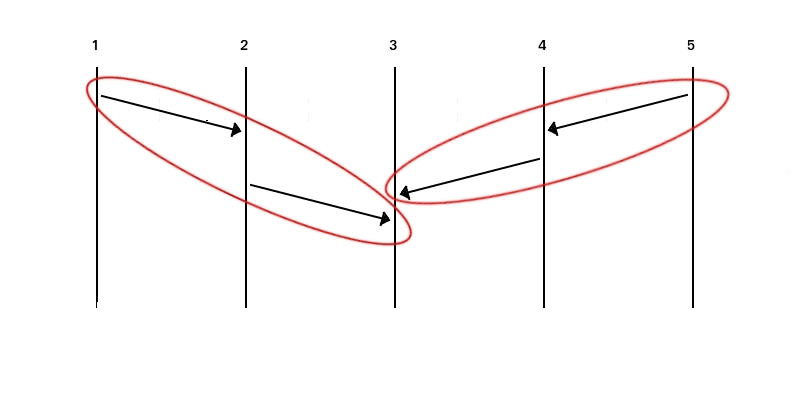
\includegraphics[width=0.5\textwidth]{fig/cut-total-ordering-partial}
  \caption{distributed program points in totally ordered subsets}
\end{figure}

%%\sc{TODO: define consistency lattice of vector clocks. talk about how all logs must be in the lattice, but the lattice itself merely gives a bound on the communication possible in the system. prove these properties with notes - prove the send/receive checksum.}

\begin{definition}[Consistent Distributed State]
    \label{def:consistent_distributed_state}Let $p_{\sigma}$, be the set of
    host states in a distributed program point $p$. Where $S$ is a
    consistent cut,  we say $\Sigma$ is consistent if.
    $\forall p, \in S, p_{\sigma} \subseteq \Sigma$.
\end{definition}



%%%%%%%%%%%%%%%%%%%%%%%%%%%%%%%%%%%%%%%%
%\begin{figure*}[t]
%    \center{\includegraphics[width=\textwidth]{fig/fig.pdf}}
%    \caption{\textbf{(a)} Five system traces (S1-S5) for a web
%        application that sells airplane tickets. Each trace consists
%        of log lines and corresponding vector clock timestamps. In the
%        traces, two clients access a single server. \textbf{(b)} A
%visualization of the five system traces as space time diagrams. Time
%flows down, and events at each host are shown in a single
%column.\label{fig:label}} \end{figure*}
%%%%%%%%%%%%%%%%%%%%%%%%%%%%%%%%%%%%%%%%

%%%%%%%%%%%%%%%%%%%%%%%%%%%%%%%%%%%%%%%%%%%%
\section{Ordering events with vector time}
\label{sec:formal-vector-clocks}
%%%%%%%%%%%%%%%%%%%%%%%%%%%%%%%%%%%%%%%%%%%%

%% We now explain the algorithm using which the
%% vector timestamps are maintained. This explanation corresponds to a
%% system that uses message passing, though vector timestamps can be used
%% for ordering event instances in a system that uses other mechanisms
%% for inter-host communication, such as shared memory.

Vector time~\cite{fidge_vector_clocks_1988,
  mattern_vector_clocks_1989} is a logical clock mechanism that
provides a partial ordering of event instances. In a distributed
system of $h$ hosts, each host maintains an array of clocks $C = [c_0,
  c_1, \dots, c_{h-1}]$, in which a clock value $c_j$ records the
local host's knowledge of (equivalently, dependence on) the local
logical time at host $j$. We denote a timestamp's $C$ clock value for
host $j$ as $C[j]$.

The hosts update their clocks to reflect the actual ordering of event
instances in the system with the following three rules:

\begin{enumerate}

    \item All hosts start with an initial vector clock value of
        $[0,\dots,0]$.

    \item When a host $i$ generates an event instance, it increments
        its own clock value (at index $i$) by 1, i.e $C_i[i]++$.

    \item When a host $h$ communicates with a host $h'$, $h$ shares
        it's current clock $C_h$ with $h'$, and $h'$ updates its local
        clock $C_{h'}$ so that $\forall i, C_{h'}[i] =
        \max\{C_h[i],C_{h'}[i]\}$. The host $h'$ also updates its local
        clock value as in (2), since message receipt is considered an
        event.

\end{enumerate}




%%%%%%%%%%%%%%%%%%%%%
\section{Logging node state}
\label{sec:logging-variables}
%%%%%%%%%%%%%%%%%%%%%

A program slice, is a subset of statements in a program, which either
affect or are affected by some root statement. Forward slicing
computes the set of statements affected by the root. Backwards slicing
computes the set of statements which affect the root. \dinv extends
Ottenstein's algorithm~\cite{Ottenstein:1984} for building a program
dependence graph (PDG) with interprocedural analysis and builds a
system dependence graph~\cite{Walkinshaw03thejava}. The roots of the
slices in Dinv are network function calls. Dinv generates the set of
variables to log by computing backwards slices from network writes and
forward slices from network reads. The general algorithm for source
code instrumentation is described in Algorithm~\ref{alg:instrument}.

Logging \emph{network interacting variables} after each executed
instruction would still produce an unmanageably large log. Dinv
resolves this by logging at just select program points. Dinv includes
two methods for identifying logging locations: a general-purpose
automated approach and an approach based on developed-supplied
annotations (Table~\ref{table:inst-strat}).

Automated dump statement injection follows a general heuristic. The
source code of the program is scanned, and annotations are injected at
the entry and exit point of each function in the program.
%
Semi-automated logging statements require the addition of annotations
by either a developer, or by automated injection. Once a program has
been annotated, \dinv analyzes the source code using program slicing,
and replaces the annotations with logging code.
Algorithm~\ref{alg:instrument} details this process at a high level.
%
Manual logging statements are specified explicitly by developers. They
specify a list of variables as arguments, and log them. This offers
fine-grained control over the instrumentation. In cases where many
variables are in scope and interact with the network the majority of
detected invariants are irrelevant to a desired system property and
obfuscate \dinv's output. We preferable when verifying invariants on
small sets of variables.

%%%%%%%%%%%%%%%%%%%%%%%%%%%%%%%%%%%%%%%%%%
\subsection{Logging functions}
\label{sec:logging-functions}
%%%%%%%%%%%%%%%%%%%%%%%%%%%%%%%%%%%%%%%%%%

One factor which complicates logging variables is their scope.
Conventionally variables are logged at a specific point in a programs
execution, this has the advantage of capturing values at a specific
moment in time, but also isolates them from being analyzed with
variables which are present in another scope. To address situations
where the variables should be logged at a specific point, and
situations where sets of variables in different scopes should be
logged together, \dinv has two distinct logging functions.

\textit{Dump} writes the values of variables directly to a log when it
is executed. Each unique dump statement is later merged as an
independent entity, the result is invariants which reflect system
invariants at arbitrary points. %Writes variables immediately to a log.

\textit{Track} writes variables to a key-value store and delays writing these
to a log until the local vector time is incremented. By deferring and
aggregating state a more complete view of a node's state can be
analyzed together, at the cost of precision.

%% The annotations for both functions are \textit{//@dump} and
%% \textit{//@track} respectively.

%%%%%%%%%%%%%%%%%%%%%%%%%%%%%%%%%%%%%%%%%%%%%%%%%%%%%%%%%%%%%%%%%
\begin{algorithm}[t]
    \KwData{Source code with dump statements $S$}
\KwResult{Instrumented Source Code $I$}

    $I$ = $S$ \\
    $dumpNode$ = CollectDumpAnnotationASTNodes($S$) \\
    \For{$dump \in dumpNodes$} {
        $variables$ = ComputeAffected($dump.line$,$S$)\\
        $loggingCode$ = NewLoggingCode($variables$, $dump.line$, $S$)\\
        $I$ += $loggingCode$\\
    }
    \Return{$Delta$}
    \caption{Algorithm converting commented logging annotation to logging code.}
    \label{alg:instrument}
\end{algorithm}
%%%%%%%%%%%%%%%%%%%%%%%%%%%%%%%%%%%%%%%%%%%%%%%%%%%%%%%%%%%%%%%%%



%%%%%%%%%%%%%%%%%%%%%%%%%%%%%%%%%%%%%%%%
\section{Constructing the lattice}
\label{sec:lattice-appendix}
%%%%%%%%%%%%%%%%%%%%%%%%%%%%%%%%%%%%%%%%

Algorithm~\ref{alg:lattice} presents the lattice construction
algorithm. Each level of the lattice is constructed sequentially.  All
clocks from the previous level have their values incremented by 1 for
each node. If the incremented clock value is valid under the
happens-before relation, it is appended to the next level of the
lattice.

%%%%%%%%%%%%%%%%%%%%%%%%%%%%%%%%%%%%%%%%%%%%%%%%%%%%%%%%%%%%%%%%%%%%%%%%%%%%%
\begin{algorithm}[t]

    \KwData{Set of Host traces $T$}
    \KwResult{Lattice representation of a System Trace $S$}
    i = 0 \;
    Level[i].append(ZeroClock())\;
    \While{!Level[i].empty()} {
        i++\;
        \For{Clock $\in$ Level[i-1]} {
            \For{Host $\in$ T}{
                Clock.increment(Host)\;
                \If {ValidLatticePoint(T,Clock)}{
                    Level[i].append(Clock)
                }
            }
        }
        $S$.append(Level[i])
    }
    \vspace{2mm}
    \caption{Lattice Construction Algorithm}
    \label{alg:lattice}
\end{algorithm}
%%%%%%%%%%%%%%%%%%%%%%%%%%%%%%%%%%%%%%%%%%%%%%%%%%%%%%%%%%%%%%%%%%%%%%%%%%%%%



%%%%%%%%%%%%%%%%%%%%%%%%%%%%%%%%%%%%%%%%%%%%%%%%%%%%%%%%
\section{Constructing strongly consistent cuts}
\label{sec:consistent-cuts-appendix}
%%%%%%%%%%%%%%%%%%%%%%%%%%%%%%%%%%%%%%%%%%%%

\textbf{Enumerating Messages}: A cut is consistent if and only if all
messages sent by nodes in a cut, were also received by a node in the
cut.  The lattice constructed in the previous section contains the set
of all possible cuts, some of which are inconsistent. If a cut is
consistent the number of in flight messages at the corresponding
vector time is zero. Checking this property can be done by iterating
through the execution logs, and counting sending and receiving events.
Because the lattice maintains the happens-before relation, If the
number of sent and received messages are equal, a cut at that time is
consistent.  Algorithm~\ref{alg:enumerate} counts the number of send
and receive events on each node by maintaining a delta of sent and
received messages.

%%%%%%%%%%%%%%%%%%%%%%%%%%%%%%%%%%%%%%%%%%%%
\begin{algorithm}[t]
    \KwData{Set of Host traces $T$}
    \KwResult{Enumerated index of Send and Receive Events $Delta$}
    \For{node $\in$ $T$} {
        \For{event $\in$ node} {
            \If{(event.WasASend())} {
                receiver, receiverEvent := logs.FindReceive(event)
                $Delta$[node][event]++
                $Delta$[receiver][receiverEvent]-\,-
            }
        }
    }
    \Return{$Delta$}
    \caption{Sent and Received message enumeration}
    \label{alg:enumerate}
\end{algorithm}
%%%%%%%%%%%%%%%%%%%%%%%%%%%%%%%%%%%%%%%%%%%


\textbf{Extracting Cuts}: The next step in the log merging process it
to process the lattice by removing all points which do not correspond
to consistent cuts.  This is done by counting all sent and received
messages at a system at each node in the lattice.  The +1 per for a
send, and -1 per a receive are stored as a \emph{delta} calculated in
the previous process. 
%
Figures~\ref{fig:time-lattice}A shows enumerated send and receive
values in red, and Figures~\ref{fig:time-lattice}B highlights the
corresponding points of the lattice which represent consistent cuts.
if the sum of the \emph{delta} for each node in a cut within the
lattice is $0$ the cut is consistent. This calculation run on each
point in the lattice produces the complete set of consistent cuts.  An
abstract version of this process can be found in
Algorithm~\ref{alg:mineCuts}.

%\begin{figure}[h]
%    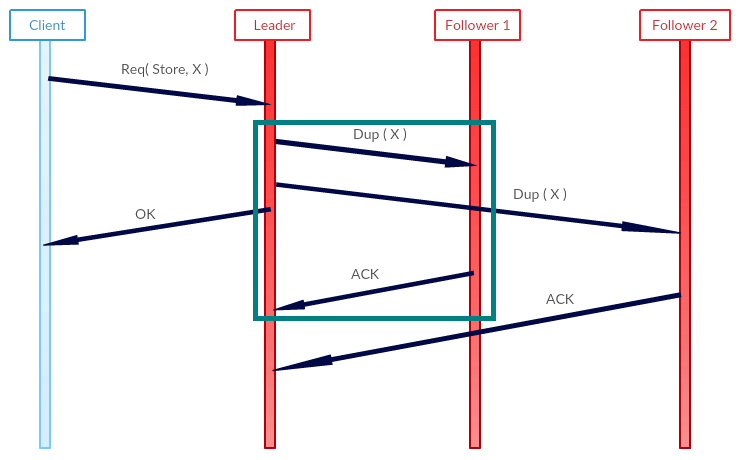
\includegraphics[width=0.5\textwidth]{fig/highlighted-lattice}
%  \caption{Subset of example execution}
%\end{figure}

\begin{algorithm}
 \KwData{$lattice$, $clocks$, $delta$}
 \KwResult{$cuts$}
 \For{$level \in lattice$} {
    \For{$node \in level$} {
        $delta$ := $0$;
        \If{$node \in clocks$} {
            \For{$node$,$clockValue$ $\in$ $node$} {
                $delta$ += $deltaComm$[$node$][$clockValue$]
            }
       }
       \If{$delta$ == $0$} {
            $cuts$.append($node$)
       }
    }
 }
 \Return{$cuts$}

    \vspace{2mm}
 \caption{Algorithm for determining which lattice points correspond to a consistent cut}
 \label{alg:mineCuts}
\end{algorithm}



%%%%%%%%%%%%%%%%%%%%%%%%%%%%%%%%%%%%%%%%%%%%
\textbf{Collecting Hosts States}: Next we collect the set of node
states  at the logical times they occurred in each consistent cut.
This computation is done by searching the execution logs for node
states with matching vector clock values.
%
One challenge is the lack of a one-to-one correspondence between node
states, and vector clock values.  This is the consequence of either
having \textit{Dump} statements log a nodes state multiple times
before incrementing its clock value, or having no dump statement
executed at the given time. In such situations we choose the logged
state based on the last networking operation performed by the node. In
the case where the last operation was a receive, the node state
corresponding to the earliest event instance is selected. Conversely
if the last operation was to send a message, the node state
corresponding to the last event instance is selected.  If no node
state is available it is not merged. In
Section~\ref{sec:logging-functions} we introduced \textit{Track}
logging functions to mitigate this complication.  \textit{Track} which
logs variables to a key value store, and only writes to a log during
increments of vector time.  Logging with a key value store has the
advantage of aggregating node state and providing a one to one
correspondence between vector time and and logged state, but has the
disadvantage of missing multiple intermediate state transitions during
a single vector time.  The output of this process is the complete set
of node states at every point during execution when all state was
resident in memory. 

\begin{figure}[h]
    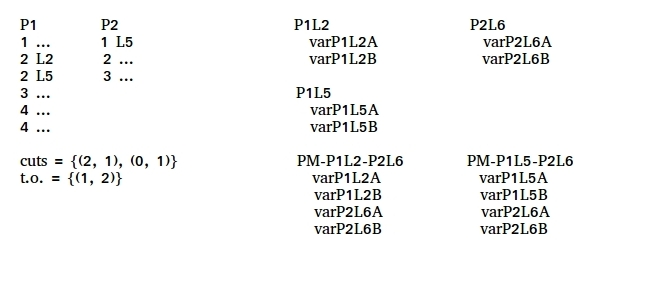
\includegraphics[width=0.5\textwidth]{fig/merge-point-logs}
  \caption{Retrieve consistent node states from logs}
\end{figure}

%%%%%%%%%%%%%%%%%%%%%%%%%%%%
\begin{algorithm}
 \KwData{$Cuts$, $Log$}
 \KwResult{Set of consistent node states $S$}
 \For{$Cut \in Cuts$} {
     \For{$Host$,$Clock \in Cut$} {
         $s$ += getHostStateFromLog($Host$,$Clock$,$Log$)
     }
     $S$.append($s$)
 }
 \Return{$S$}

 \caption{Collect the Host's state, for each consistent cut}
 \label{alg:collectStates}
\end{algorithm}
%%%%%%%%%%%%%%%%%%%%%%%%%%%%



%%%%%%%%%%%%%%%%%%%%%%%%%%%%%%%%%%%%%%%%%%%
\section{Daikon background}
\label{daikon-appendix}
%%%%%%%%%%%%%%%%%%%%%%%%%%%%%%%%%%%%%%%%%%%

Daikon is a dynamic analysis tool which automatically detects likely
data invariants in sequential systems. Daikon derives data invariants
by processing data traces (\emph{dtraces}) produced during the run
time of a program. A trace consists of a set of variable names, and
the various values they took over the course of a programs
execution. To produce a system trace Daikon injects logging statements
at the beginning and end of both functions and loops, which dump the
values of all variables in scope. Daikon uses a confidence measure to
filter our spurious invariants.

\begin{lstlisting}[
    caption={simple program with loop invariants},
    label={lst:loopinvariants}
    ]
i := 0
j := 1
k := i + j
for i < 5 {
    k = i + j
    i++
    j++
}
\end{lstlisting}

\begin{lstlisting}[
    caption={Code instrumented to produce trace},
    label={lst:insturmenteddaikonLoop}
    ]
i := 0
j := 1
k := i + j
for i < 5 {
    logToTrace(i,j,k)
    k = i + j
    i++
    j++
    logToTrace(i,j,k)
}
\end{lstlisting}

\begin{table}
        \caption{Daikon Invariants}
        \label{table:daikon-invariants}
    \begin{framed}
        \begin{enumerate}[noitemsep]
                \item $k = i + j$
                \item $j > i$
                \item $j = i + 1$
                \item $i < 5$
        \end{enumerate}
   \end{framed}
\end{table}

%%%%%%%%%%%%%%%%%%%%%%%%%%%%%%%%%%%%%%%%%%%
\subsection{Translation Daikon invariants to first order logic}
\label{sec:daikon-to-fol}
%%%%%%%%%%%%%%%%%%%%%%%%%%%%%%%%%%%%%%%%%%%

Daikon supports unary, binary, and ternary invariants out of the box,
and does not support predicate logic.  The result of this is that
invariant properties that hold over sets of $n$ variables are output
in pieces. For example if 4 variables $X_0 \dots X_3$ were determined
to always be equal Daikon's output would appear as $X_0 == X_1$, $X_0
== X_2$, $X_0 == X_3$. In this case the 4 invariants can be combined
transitively to show equality among all of them. In such cases we
present the invariant as a first order logical formula. For example in
this case the invariant would be denoted $\forall i,j$, $X_i = X_j$.

In other cases an invariant property is that in a single case a
property exists. As an example in Section~\ref{sec:application} we
espouse the strong leadership principle of raft, stating that only a
leader is able to issue an append entries message, and should
therefore have a log greater than or equal to each of the followers.
In this case we logged host state in two separate functions, one for
followers, and one for the leader. The Daikon output from the
execution was a separate file for each host which was a leader during
execution. Detailed in Table~\ref{table:Existance-Invariant} is the
set of invariants used to support the property of strong leadership in
etcd raft. The table supposes a cluster was composed of 3 hosts
$A$,$B$,$C$ each of which became a leader at least once. From the
output it can be inferred that If a host is in the state leader, it
has a log larger than that of the followers, and the followers have
logs of equal size. For conciseness we represent this invariant with the following formula $Leader-LogSize >= Followers-LogSize $,$\forall followers$.

\begin{table}
        \caption{Raft Strong Leadership Invariant}
        \label{table:Existance-Invariant}
    \begin{framed}
        \caption{File A-Leader B-Follower C-Follower}
        \begin{enumerate}[noitemsep]
                \item $A-State == Leader$
                \item $C-State == B-State$
                \item $B-State == Follower$
                \item $A-LogSize >= B-LogSize$
                \item $A-LogSize >= C-LogSize$
                \item $B-LogSize == C-LogSize$
        \end{enumerate}
        \caption{File A-Follower B-Leader C-Follower}
        \begin{enumerate}[noitemsep]
                \item $B-State == Leader$
                \item $A-State == C-State$
                \item $A-State == Follower$
                \item $B-LogSize >= A-LogSize$
                \item $B-LogSize >= C-LogSize$
                \item $A-LogSize == C-LogSize$
        \end{enumerate}
        \caption{File A-Follower B-Follower C-Leader}
        \begin{enumerate}[noitemsep]
                \item $C-State == Leader$
                \item $A-State == B-State$
                \item $B-State == Follower$
                \item $C-LogSize >= B-LogSize$
                \item $C-LogSize >= A-LogSize$
                \item $B-LogSize == A-LogSize$
        \end{enumerate}
   \end{framed}
\end{table}



\balance
\bibliographystyle{abbrv}
\bibliography{paper}

\end{document}
